\documentclass[11pt,a4paper]{book}
\usepackage[english,spanish]{babel}
\spanishdecimal{.}
\usepackage{tkz-fct}
\usepackage{tkz-euclide}
% \usepackage{biblatex}
\usepackage{indentfirst}
% \setlength{\parindent}{15pt}
\usepackage[utf8]{inputenc}
\usepackage{graphicx}
\usepackage[T1]{fontenc}
\usepackage{anysize} % Soporte para el comando \marginsize
%\marginsize{1.5cm}{1.5cm}{0.5cm}{1cm}
% \marginsize{2.5cm}{1.5cm}{2.5cm}{2.5cm} %left/right/top/bottom  Usual
\marginsize{2.5cm}{2.5cm}{2.7cm}{2.7cm} %left/right/top/bottom
\usepackage{float}
\usepackage[pagestyles]{titlesec}
\usepackage{amssymb}
\usepackage{listings}
\usepackage{caption}
\usepackage{subcaption}
\usepackage{amssymb}
\usepackage{amsfonts}
\usepackage{amsmath}
\usepackage{amsthm}
\usepackage{dsfont}
\usepackage{bbm}
\usepackage{textcomp}
\usepackage{stmaryrd}
\usepackage{xcolor}
\usepackage{tkz-fct}
\usepackage{tkz-euclide}
\usepackage{parskip}
\newcommand{\code}[1]{\texttt{#1}}
%%%%%%%%%%%%%%%%%%%%%%%%%%%%%%%%%%%%%%%%%%%%%%%%%%%%%%%%%%%%%%%%%%%%%%%%%%%%%%%%
%%%%%%%%%%%%%%%%%%%%%%%%%%%%%%%%%%%%%%%%%%%%%%%%%%%%%%%%%%%%%%%%%%%%%%%%%%%%%%%%
\usepackage[pagewise]{lineno}
\usepackage{csquotes}
\usepackage[backend=biber,style=alphabetic]{biblatex}
\nocite{*}
% Add Line Comment	Ctrl+K Ctrl+C	editor.action.addCommentLine
% Remove Line Comment	Ctrl+K Ctrl+U	editor.action.removeCommentLine
%%%%%%%%%%%%%%%%%%%%%%%%%%%%%%%%%%%%%%%%%%%%%%%%%%%%%%%%%%%%%%%%%%%%%%%%%%%%%%%%
%%%%%%%%%%%%%%%%%%%%%%%%%%%%%%%%%%%%%%%%%%%%%%%%%%%%%%%%%%%%%%%%%%%%%%%%%%%%%%%%
\bibliography{Bibliography.bib}
\usepackage{float}
\usepackage{mathrsfs}
% \usepackage{lineno,hyperref}
% \usepackage[colorlinks=true, allcolors=blue]{hyperref}
\usepackage{hyperref}
\hypersetup{
    colorlinks=true,
    linkcolor=blue,
    filecolor=magenta,      
    urlcolor=cyan,
    pdftitle={Proyecto de Tesis III},
    pdfpagemode=FullScreen,
    }
\usepackage{blindtext}
\usepackage{xcolor}
\newenvironment{abstract}[1]
  {\bigskip\selectlanguage{#1}%
   \begin{center}\bfseries\Large\abstractname\end{center}}
  {\par\bigskip}
%\linespread{1} \sloppy
\usepackage{multicol}
\usepackage{multirow}
% \renewcommand{\thepage}{}
\columnsep=7mm
\pagestyle{plain}
%%%%%%%%%%%%%%%%%%%%%%%%%%%%%%%%%%%%%%%%%%%%%%%%%%%%%%%%%%%%%%%%%%%%%%%%%%%%%%%%
%%%%%%%%%%%%%%%%%%%%%%%%%%%%%%%%%%%%%%%%%%%%%%%%%%%%%%%%%%%%%%%%%%%%%%%%%%%%%%%%
% Headstyle and footstyle


% \usepackage[most]{tcolorbox} 
% \titleformat{\chapter}[display] 
% {\bfseries\Large\itshape}{\vspace{-3cm} \color{gray} Capitulo N° \ \thechapter}{-2.5ex} 
% {
%    %  \color{black}
%    % \rule{\textwidth}{1pt}
%    % \vspace{1ex}
%    %  \centering
% }[\vspace{-3.5ex}\rule{\textwidth}{0.3pt}\vspace{-0.7cm}] 

\usepackage{fancyhdr}
\usepackage{blindtext}
\usepackage{lastpage}

\pagestyle{fancy}
\fancyhead{} 
\setlength{\headheight}{30pt}
\rhead[\textcolor{black}{\leftmark}]{
\includegraphics[scale=0.02]{Carátula/Uni-logo_transparente.png}}
\lhead[\textcolor{black}{UNI}]{\textcolor{black}{\rightmark}}
\fancyfoot{}
\lfoot[\textcolor{black}{\thepage}]{\textcolor{black}{Facultad De Ciencias}}
%\fancyfoot[R]{Facultad De Ciencias (EPM)}
\rfoot[\textcolor{black}{Escuela Profesional de Matemática}]{\textcolor{black}{\thepage}}

\renewcommand{\headrulewidth}{0.9pt}
\renewcommand{\footrulewidth}{0.5pt}
\let\HeadRule\headrule
\let\FootRule\footrule
\renewcommand\headrule{\color{black}\HeadRule}
\renewcommand\footrule{\textcolor{black}{\FootRule}}

% \fancypagestyle{chapterfancy}{%
    \pagestyle{fancy}
    
    \fancyfoot{}
    \lfoot[\textcolor{black}{\thepage}]{\textcolor{black}{Facultad De Ciencias}}
    %\fancyfoot[R]{Facultad De Ciencias (EPM)}
    \rfoot[\textcolor{black}{Escuela Profesional de Matemática}]{\textcolor{black}{\thepage}}
% }
 \renewcommand{\chaptermark}[1]{\markboth{#1}{}}
 
% \makeatletter
% \renewcommand\chapter{\if@openright\cleardoublepage\else\clearpage\fi
%                     \thispagestyle{chapterfancy}% original style: plain
%                     \global\@topnum\z@
%                     \@afterindentfalse
%                     \secdef\@chapter\@schapter}
% \makeatother
%%%%%%%%%%%%%%%%%%%%%%%%%%%%%%%%%%%%%%%%%%%%%%%%%%%%%%%%%%%%%%%%%%%%%%%%%%%%%%%%
%%%%%%%%%%%%%%%%%%%%%%%%%%%%%%%%%%%%%%%%%%%%%%%%%%%%%%%%%%%%%%%%%%%%%%%%%%%%%%%%

%New colors defined below
\definecolor{codegreen}{rgb}{0,0.6,0}
\definecolor{codegray}{rgb}{0.5,0.5,0.5}
\definecolor{codepurple}{rgb}{0.58,0,0.92}
\definecolor{backcolour}{rgb}{0.95,0.95,0.92}

%Code listing style named "mystyle"
\lstdefinestyle{mystyle}{
  backgroundcolor=\color{backcolour}, commentstyle=\color{codegreen},
  keywordstyle=\color{magenta},
  numberstyle=\tiny\color{codegray},
  stringstyle=\color{codepurple},
  basicstyle=\ttfamily\footnotesize,
  breakatwhitespace=false,         
  breaklines=true,                 
  captionpos=b,                    
  keepspaces=true,                 
  numbers=left,                    
  numbersep=5pt,                  
  showspaces=false,                
  showstringspaces=false,
  showtabs=false,                  
  tabsize=2
}

%"mystyle" code listing set
\lstset{style=mystyle}

%%%%%%%%%%%%%%%%%%%%%%%%%%%%%%%%%%%%%%%%
% This version enumerates each newtheorem environment as they were independent
% \newtheorem{teorema}{Teorema}[section]
% % \newtheorem{prueba}{Prueba}[section]
% % \newtheorem{prueba*}{Prueba}[section]
% \newtheorem{corolario}{Corolario}[section]
% \newtheorem{observacion}{Observaci\'on}[section]
% \newtheorem{lema}{Lema}[section]
% % \newtheorem{algoritmo}{Algoritmo}[section]
% \newtheorem{proposicion}{Proposici\'on}[section]

% \theoremstyle{definition}%Not upshape
% \newtheorem{definicion}{Definici\'on}[section]
% \newtheorem{notacion}{Notaci\'on}[section]
% \newtheorem{ejemplo}{Ejemplo}[section]
% \newtheorem{solucion*}{Soluci\'on}[section]
%%%%%%%%%%%%%%%%%%%%%%%%%%%%%%%%%%%%%%%%
% \makeatletter
% % \def\thm@headpunct{:} % Cambiar el símbolo después del título
% \def\thm@notefont{\bfseries} % Hacer en negrita las notas opcionales
% \makeatother
%%%%%%%%%%%%%%%%%%%%%%%%%%%%%%%%%%%%%%%%
% This version enumerates each newtheorem environment respecting order
\newtheorem{teorema}{Teorema}[section]
% \newtheorem{prueba}{Prueba}[section]
% \newtheorem{prueba*}{Prueba}[section]
\newtheorem{corolario}[teorema]{Corolario}
\newtheorem{observacion}[teorema]{Observaci\'on}
\newtheorem{lema}[teorema]{Lema}
% \newtheorem{algoritmo}{Algoritmo}[section]
\newtheorem{proposicion}[teorema]{Proposici\'on}

\theoremstyle{definition}%Not upshape
\newtheorem{definicion}[teorema]{Definici\'on}
\newtheorem{notacion}[teorema]{Notaci\'on}
\newtheorem{ejemplo}[teorema]{Ejemplo}
\newtheorem{solucion*}[teorema]{Soluci\'on}
%%%%%%%%%%%%%%%%%%%%%%%%%%%%%%%%%%%%%%%%
\linespread{1.25} \sloppy %Interlineado
\newcommand{\datainset}{\mathcal{X}}
\newcommand{\dataoutset}{\mathcal{Y}}
\newcommand{\MSE}{\overline{\mathcal{E}^2}}
\newcommand{\setcomplement}{\mathsf{c}}
\newcommand{\R}{\mathbf{R}}
\newcommand{\N}{\mathbf{N}}
\newcommand{\C}{\mathbb{C}}
\newcommand{\Lr}{\mathcal{L}}
\newcommand{\Model}{\mathcal{M}}
% \newcommand{\fc}{\displaystyle\frac}
\newcommand{\ds}{\displaystyle}
\newcommand{\Ker}{\textup{Ker}}
\newcommand{\Imagesymb}{\textup{Im}}
\newcommand{\Span}{\textup{span}}
\newcommand{\rank}{\textup{rank}}
% \newcommand{\fixedrisk}{\mathcal{E}_R}
%%%%%%%%%%%%%%%%%%%%%%%%%%%%%%%%%%%%%%%%%%%%%%%%%%%%%%%%%%%%%%%%%
%Solo simbolos
\newcommand{\empiricalrisksymb}{\hat{\mathcal{R}}}
\newcommand{\empiricalcovmat}{\hat{\Sigma}}
\newcommand{\fixedrisksymb}{\mathcal{R}}
\newcommand{\epigraphsymb}{\textup{epi}}
\newcommand{\EVsymb}{\mathbb{E}}
\newcommand{\Probsymb}{\mathds{P}}
\newcommand{\RSSsymb}{\textsf{RSS}}
\newcommand{\suppsymb}{\textup{supp}}
\newcommand{\Proysymb}{\textup{Proy}}
\newcommand{\Real}{\mathbb{R}}
\newcommand{\Integer}{\mathbb{Z}}
\newcommand{\Natural}{\mathbb{N}}
\newcommand{\penaltymsymb}{\textup{pen}}
\newcommand{\Varsymb}{\textup{\textsf{Var}}}
\newcommand{\Covsymb}{\textup{\textsf{Cov}}}
\newcommand{\CVsymb}{\empiricalrisksymb_{\textup{cv}}}
\newcommand{\indicator}{\boldsymbol{\mathds{1}}}
\newcommand{\expsymb}{\textup{exp}}
\DeclareMathOperator{\tr}{tr}% \newcommand{\transpose}{\ensuremath{{\scriptscriptstyle{T}}}}
\DeclareMathOperator{\Dom}{\text{Dom}}
\DeclareMathOperator*{\argmax}{\text{arg máx}}
\DeclareMathOperator*{\argmin}{\text{arg mín}}
%%%%%%%%%%%%%%%%%%%%%%%%%%%%%%%%%%%%%%%%%%%%%%%%%%%%%%%%%%%%%%%%%
%Con argumentos
\newcommand{\empiricalrisk}[1]{\hat{\mathcal{R}}\left( #1 \right)} % Check changes on document after 30/10/2024 cuz before it was the same as fixedrisk
\newcommand{\fixedrisk}[1]{\mathcal{R}\left( #1 \right)}
\newcommand{\epigraph}[1]{\textup{epi}\left( #1 \right)}
\newcommand{\RSS}[1]{\textsf{RSS}\left( #1 \right)}
\newcommand{\supp}[1]{\textup{supp}\left( #1 \right)}
\newcommand{\Proy}[2]{\textup{Proy}_{#1} {#2}} 
\newcommand{\EV}[1]{\mathbb{E}\left[#1\right]}
\newcommand{\EVX}[2]{\mathbb{E}_{#1} \left[ #2 \right]}
\newcommand{\Prob}[1]{\mathds{P}\left( #1 \right)}
\newcommand{\penaltym}[1]{\textup{pen} \left( #1 \right)}
\newcommand{\card}[1]{\text{\textsf{n}}\left( #1 \right)}
\newcommand{\abs}[1]{\left| #1 \right|}
\newcommand{\differential}{\operatorname{d\!}}
\newcommand{\floor}[1]{\left\lfloor #1 \right\rfloor}
\newcommand{\ceil}[1]{\left\lceil #1 \right\rceil}
\newcommand{\Var}[1]{\textup{\textsf{Var}}\left(#1\right)}
\newcommand{\Cov}[2]{\textup{\textsf{Cov}}\left(#1,#2\right)}
\newcommand{\innerdot}[2]{\left\langle#1,#2\right\rangle}
\newcommand{\intsequenceto}[1]{\llbracket #1 \rrbracket}
\newcommand{\CV}[1]{\empiricalrisksymb_{\textup{cv}}\left(#1\right)}
\newcommand{\trace}[1]{\tr\left( #1 \right)}
\newcommand{\Image}[1]{\textup{Im}\left(#1\right)}
\renewcommand{\exp}[1]{\textup{exp}\left(#1\right)}
%%%%%%%%%%%%%%%%%%%%%%%%%%%%%%%%%%%%%%%%%%%%%%%%%%%%%%%%%%%%%%%%%
%%%%%%%%%%%%%%%%%%%%%%%%%%%%%%%%%%%%%%%%
\renewcommand{\thefootnote}{\fnsymbol{footnote}}

%%%%%%%%%%%%%%%%%%%%%%%%%%%%%%%%%%%%%%%%
%%%%%%%%%%%%%%%%%%%%%%%%%%%%%%%%%%%%%%%%
%%%%%%%%%%%%%%%%%%%%%%%%%%%%%%%%%%%%%%%%
\usepackage{titlesec}


% \titleformat{\chapter}[display]
%   {\Huge\bfseries}{}{0pt}{\thechapter \quad\Huge}                % Space between number and title
%       {}  
%%%%%%%%%%%%%%%%%%%%%%%%%%%%%%%%%%%%%%%%
%%%%%%%%%%%%%%%%%%%%%%%%%%%%%%%%%%%%%%%%
%%%%%%%%%%%%%%%%%%%%%%%%%%%%%%%%%%%%%%%%



\begin{document}
    \renewcommand{\listtablename}{Índice de tablas}
    \renewcommand{\tablename}{Tabla}
    %%%%%%%%%%%%%%%%%%%%%%%%%%%%%%%%%%%%%%%%
    \thispagestyle{empty}
    \addtocounter{page}{-1}
    \begin{center}
        {\huge \textbf{UNIVERSIDAD NACIONAL DE INGENIERÍA}}\\
    \vspace{0.5cm}
        {\huge \textbf{FACULTAD DE CIENCIAS}}\\
    \vspace{0.25cm}
    {\huge \textbf{Escuela Profesional de Matemática}}\\
    \vspace{0.25cm}
        \begin{figure}[h!]
            \centering
            
\includegraphics[scale=0.15]{Carátula/Uni-logo_transparente.png}
        \end{figure}
    \vspace{0.1cm}
         {\huge \textbf{Informe de prácticas pre-profesionales}}\\
    \vspace{1cm}
    {\huge \textbf{``Análisis exploratorio de los datos de asistencia a clases de reforzamiento de los estudiantes de la Universidad Tecnológica del Perú''}}\\
    \vspace{1cm}
        \LARGE{\textbf{Realizado en: }Universidad Tecnológica del Perú}\\
        \LARGE{\textbf{Tema: }Tutoría}
    \end{center}
    \vspace{1cm}
    
    \begin{center}
        \LARGE{\textbf{Por: }Jael David Laiza Gomez}\\
        \LARGE{\textbf{Código: }20204038K}
    \vspace{1cm}
    
    \date{\LARGE{\today}}
    \makeatletter
    \@date
    \makeatother
    \end{center}
    %%%%%%%%%%%%%%%%%%%%%%%%%%%%%%%%%%%%%%%%
    
    %%%%%%%%%%%%%%%%%%%%%%%%%%%%%%%%%%%%%%%%
    \tableofcontents
    %%%%%%%%%%%%%%%%%%%%%%%%%%%%%%%%%%%%%%%%

    %%%%%%%%%%%%%%%%%%%%%%%%%%%%%%%%%%%%%%%%
    \chapter*{Resumen}\addcontentsline{toc}{chapter}{Resumen}
        El contenido principal del informe se centra en realizar un análisis exploratorio de los datos obtenidos a partir de las sesiones de talleres y tutorías dictadas a los estudiantes de la \textit{Universidad Tecnológica del Perú}, con el fin de determinar si existen variables aleatorias que modelen el comportamiento estadístico de los datos. Se presenta el esquema matemático del modelo y los resultados experimentales obtenidos a partir de los datos usando \textsc{Power BI}, \textsc{PowerQuery} y \textsc{Python}.
    \chapter*{Introducción}\addcontentsline{toc}{chapter}{Introducción}
        El presente informe corresponde a las Prácticas Pre-Profesionales realizadas en la
        Universidad Tecnológica del Perú (UTP), desde el 3 de marzo de 2025 hasta el 2 de agosto de 2025.
        
        La empresa Universidad Tecnológica del Perú se dedica a formar profesionales en áreas como ingeniería, arquitectura, ciencias de la salud, ciencias sociales y ciencias de la comunicación.
        
        En particular, la sede en cuestión a tratar (\textit{UTP - Lima Centro}) está localizada en \textit{Av. Arequipa 265, Lima 15046}.
        
    \chapter*{Antecedentes}\addcontentsline{toc}{chapter}{Antecedentes}
        En la Universidad Tecnológica del Perú, en vista de la necesidad de brindar apoyo académico a los estudiantes en cursos de matemática o física se realizan sesiones extracurriculares para todos los estudiantes que se clasifican en \textit{talleres} y \textit{tutorías}. Las sesiones son no obligatorias, por lo que los estudiantes pueden optar por inscribirse o no a este tipo de actividad y, estando inscritos, pueden o no optar por asistir. Estas sesiones pueden ser dictadas en forma \textit{presencial} o \textit{virtual} (mediante la plataforma \textbf{\textit{Zoom}}).
        
        El objetivo general en ambos tipos de sesiones es la de apoyar a los estudiantes en la resolución de problemas relacionados a los temas vistos en las clases de los correspondientes cursos. Sin embargo, la diferencia entre ambos tipos de sesiones radica en el tiempo y el alcance.
        
        Por ejemplo, los \textit{talleres} presentan una duración de $90\,\textup{min}$ y un alcance máximo de hasta $100$ alumnos, mientras que las \textit{tutorías} presentan una duración de $45\,\textup{min}$ y un alcance máximo de hasta $5$ alumnos. Usualmente esto permite que un \textit{taller} se enfoque principalmente en el desarollo de la solución de problemas mientras que una \textit{tutoría} tiene un enfoque más personalizado para el alumno.

        Hasta este punto, si bien las variables más resaltantes podrían ser las del número de alumnos inscritos y el número de alumnos asistentes, si deseasemos realizar un análisis de demanda por curso, fecha y hora podria no ser suficiente. De hecho, estas últimas tendrían que ser variables que formen parte del análisis.

        Dado que se encuentran datos más detallados para las sesiones dictadas en forma \textit{virtual}, tales como datos de todas las variables mencionadas en el párrafo anterior, se considerará esto como fuente principal para el análisis exploratorio de los datos. Asimismo, se presenta la construcción matemática del problema a estudiar mediante el uso de notaciones y resultados conocidos.          
            
        \chapter{Objetivos}
            \section{Generales}
                \begin{itemize}
                    \item Realizar un análisis exploratorio de los datos de asistencia y rendimiento de cursos dictados.
                    \item Determinar si existen variables aleatorias que modelen el comportamiento estadístico de los datos.
                    \item Estudiar mediante modelos matemáticos la relación entre variables.
                \end{itemize}
            \section{Específicos}
                \begin{itemize}
                    \item Realizar un proceso ETL simple para analizar los datos de asistencia de alumnos a sesiones.
                    \item Mostrar gráficos de barras en relación a los cursos y tipos de sesiones dictadas.
                    \item Determinar la distribución del número de alumnos inscritos a sesiones (análisis por curso y global).
                    \item Determinar la distribución del número de alumnos asistentes a sesiones (análisis por curso y global).
                    \item Determinar la relación entre el número de alumnos inscritos y el número de alumnos asistentes a sesiones (análisis por curso y global).
                    \item Determinar la distribución del número de alumnos asistentes dado un número dado el número de alumnos asistentes (análisis por curso y global).
                \end{itemize}
        \chapter{Fundamento teórico}
            \section{Modelo matemático}
            Antes de estudiar las variables del problema, las planteamos matemáticamente. Para ello presentamos notaciones adecuadas y convenientes para este contexto.

            \begin{notacion}
                Denotamos al conjunto de enteros en el intervalo $I\subset\Real$ como $I_\mathbb{Z}:=I\cap\mathbb{Z}$.
            \end{notacion}
            
            \begin{definicion}[Fecha y hora]
                Denotamos al conjunto de todas las fechas representables (en un ordenador) como
                \begin{equation*}
                    \mathcal{D}:=\{(y,m,d):y\in [1900;2099]_\Integer, m\in[1;12]_\Integer, d\in D(y,m)\}
                \end{equation*}
                donde $D(y,m)\subset[1,31]_\Integer$ es el conjunto de días en el mes $m$ y año $y$. Además, definimos el conjunto de horas del día (con precisión de minutos) como
                \begin{equation*}
                    \mathcal{H}:=24\Integer\times 60\Integer
                \end{equation*}
            \end{definicion}
            
            \begin{definicion}[Cursos]
                Definimos el conjunto de cursos como
                \begin{equation*}
                    \mathcal{C}:=\{c_i: i=1,\ldots,n\}
                \end{equation*}
                para algún $n\in\mathbb{N}$, donde cada $c_i$ representa el nombre textual (o algún tipo de identficador numérico) de un curso.
            \end{definicion}

            \begin{definicion}[Tipo de sesión]
                Definimos el conjunto de los tipos de sesiones como
                \begin{equation*}
                    \mathcal{T}_\mathcal{S}:=\{\textup{Taller},\textup{Tutoría}\}
                \end{equation*}
                cuyos elementos representan el nombre textual de los tipos de sesiones.
            \end{definicion}

            \begin{definicion}[Sesión]
                Definimos el conjunto de sesiones como
                \begin{equation*}
                    \mathcal{S}:=\{s\mid s=(t_s,c_s,d_s,h_s),t_s\in\mathcal{T}_\mathcal{S},\enspace c_s\in \mathcal{C},d_s\in\mathcal{D}_\mathcal{S},h_s\in\mathcal{H}_\mathcal{S}\}
                \end{equation*}
                donde $\mathcal{D}_\mathcal{S}\subset\mathcal{D}$ y $\mathcal{H}_\mathcal{S}\subset\mathcal{H}$.
            \end{definicion}

            \begin{definicion}[Número experimental de alumnos inscritos y asistentes]
                Sea $s\in\mathcal{S}$ una sesión, definimos el par inscritos-asistentes de la sesión $s$ como $\#s:=(I_s,A_s)\in\Natural_0^2$ siendo $I_s$ el número (experimental) de inscritos y $A_s$ el número (experimental) de asistentes.
            \end{definicion}

            \begin{definicion}[Número aleatorio de alumnos inscritos y asistentes]
                Definimos el número de alumnos inscritos como la variable aleatoria $\mathcal{I}:\Omega\longrightarrow \Natural_0$ y el número de alumnos asistentes como la variable aleatoria $\mathcal{A}:\Omega\longrightarrow \Natural_0$.
            \end{definicion}

            En principio, $\mathcal{I}$ y $\mathcal{A}$ son variables aleatorias con distribuciones desconocidas. Sin embargo, dado el contexto del problema, podemos aproximar sus distribuciones a partir de los datos obtenidos.

            La aproximación es posible gracias a la ley fuerte de los grandes números (Teorema \ref{large numbers strong}), pues resulta de una aplicación particular a una variable aleatoria.

            \begin{ejemplo}[Aproximación de la distribución de probabilidad]\label{montecarlo dist prob}
                Sea $Y:\Omega\longrightarrow\mathbb{R}$ una variable aleatoria y sea $X_1,X_2,X_3,\ldots$ una sucesión de variables aleatorias independientes e idénticamente distribuidas con $X_i \sim Y$. Dado $A\subset \mathbb{R}$ fijo, determinamos la distribución de $\mathds{1}_A (X_i)$ como
                \begin{equation*}
                    \Prob{\mathds{1}_A (X_i) = x} = \left\{ \begin{array}{cl}
                         \Prob{Y \in A}&,\enspace x=1  \\
                         \Prob{Y \in A^\setcomplement}&,\enspace x=0
                    \end{array}\right.
                \end{equation*}
                De aquí, es claro que $\EV{\mathds{1}_A (X_i)}=\Prob{Y \in A}<\infty$ y si definimos
                \begin{equation*}
                    \overline{Z}_n = \frac{1}{n}\sum_{i=1}^n \mathds{1}_A (X_i),\enspace n \in\Natural
                \end{equation*}
                entonces por la ley fuerte de los grandes números se obtiene
                \begin{equation*}
                    \Prob{ \lim_{n \to \infty} \overline{Z}_{n} = \EV{\mathds{1}_A (X_i)}}= 1 \Longrightarrow \Prob{ \lim_{n \to \infty} \frac{1}{n}\sum_{i=1}^n \mathds{1}_A (X_i) = \Prob{Y \in A}}= 1
                \end{equation*}
                Esto último permite fundamentar el por qué funciona el método de Montecarlo para aproximar la distribución de una variable aleatoria. En la práctica, esto es típicamente aplicado mediante histogramas sobre un conjunto de datos.
                
                Lo que nos dice es que si deseamos aproximar $\Prob{Y \in A}$ podemos realizar $n$ experimentos tal que en cada uno de estos registremos el valor obtenido de la variable aleatoria $X_i$, luego procederíamos a contabilizar cuántas veces sucede $X_i\in A$ y finalmente nuestra aproximación sería 
                \begin{equation}\label{approx dist va montecarlo}
                    \Prob{Y \in A} \approx \frac{1}{n}\sum_{i=1}^n \mathds{1}_A (X_i)
                \end{equation}
                para un $n$ suficientemente grande. Es decir que a más experimentos mejor será la aproximación.
            \end{ejemplo}
            Ahora, con \ref{approx dist va montecarlo} estamos en condiciones de poder realizar las aproximaciones necesarias para el análisis exploratorio de los datos.
            \begin{observacion}\label{aprox fundamental}
                Aproximamos las distribuciones de $\mathcal{I}$ y $\mathcal{A}$ mediante
                \begin{equation}\label{Inscritos-Asistentes Montecarlo}
                    \Prob{\mathcal{I}=n}\approx \dfrac{\sum_{s\in \mathcal{S}} \mathds{1}_{\{n\}}(I_s)}{\card{\mathcal{S}}},\quad \Prob{\mathcal{A}=n}\approx \dfrac{\sum_{s\in \mathcal{S}} \mathds{1}_{\{n\}}(A_s)}{\card{\mathcal{S}}}
                \end{equation}
                para $\card{\mathcal{S}}$ suficientemente grande. Esto representa un método de aproximación mediante Montecarlo.
            \end{observacion}

            Como $\card{\mathcal{S}}$ representa la cantidad de sesiones (o el tamaño de $\mathcal{S}$), al referirnos a que este sea \textit{suficientemente grande} damos por entendido que a mayor cantidad de sesiones existentes mayor será la calidad de la aproximación.

            \begin{definicion}[Otras variables aleatorias]
                Definimos las variables aleatorias
                \begin{itemize}
                    \item $T_\mathcal{S}:\Omega\longrightarrow \mathcal{T}_\mathcal{S}$, tipo de sesión;
                    \item $C:\Omega\longrightarrow \mathcal{C}$, curso;
                    \item $D_\mathcal{S}:\Omega\longrightarrow \mathcal{D}$, fecha;
                    \item $H_\mathcal{S}:\Omega\longrightarrow \mathcal{H}$, hora.
                \end{itemize}
            \end{definicion}
            Debemos hacer la distinción entre estas variables aleatorias y sus homónimos definidos anteriormente, ya que estos últimos son objetos fijos. Nuevamente, asumimos que podemos aproximar sus distribuciones mediante una aproximación de Montecarlo como en \ref{Inscritos-Asistentes Montecarlo}.

            \begin{notacion}
                Denotamos $\hat{\Probsymb}_A(k):=\dfrac{\sum_{s\in \mathcal{S}} \mathds{1}_{\{k\}}(a_s)}{\card{\mathcal{S}}}$ para $k\in A$ y $a_s\in A$ una de las componentes de $s\in\mathcal{S}$.
            \end{notacion}

            \begin{observacion}
                Aproximamos las distribuciones de $T_\mathcal{S}$, $C$, $ D_\mathcal{S}$ y $H_\mathcal{S}$ mediante
                \begin{equation}\label{Otras variables aleatorias Montecarlo}
                    \Prob{T_\mathcal{S}=t}\approx \hat{\Probsymb}_{\mathcal{T}_\mathcal{S}}(t),\quad \Prob{C=c}\approx \hat{\Probsymb}_\mathcal{C}(c), \quad \Prob{D_\mathcal{S}=d}\approx \hat{\Probsymb}_{\mathcal{D}_\mathcal{S}}(d),\quad \Prob{H_\mathcal{S}=h}\approx \hat{\Probsymb}_{\mathcal{H}_\mathcal{S}}(h)
                \end{equation}
                para $\card{\mathcal{S}}$ suficientemente grande. Esto representa un método de aproximación mediante Montecarlo.
            \end{observacion}
        \section{Estimaciones}
            Hasta este punto tenemos modeladas las variables en forma matemática, sin embargo, es requerido tener datos experimentales para obtener conclusiones. De hecho, el conjunto $\mathcal{S}$ representa el conjunto de datos obtenidos en este contexto, por lo que tener un $\mathcal{S}$ suficientemente grande permitiría obtener mejores aproximaciones de las distribuciones de probabilidad.

            Más exactamente, $\mathcal{S}$ representa el conjunto de datos de las sesiones dictadas en modalidad virtual y para obtener estos datos es necesario realizar su respectiva extracción. (La etapa de extracción se detallará posteriormente).

            \begin{observacion}\label{obs prob cond}
                La distribución de probabilidad de la variable aleatorias número de inscritos en un curso dado es simplemente la probabilidad condicionada de $\mathcal{I}$ dado $C$. Por ejemplo, si deseamos calcular la probabilidad de que hayan $n$ inscritos en el curso $c$ calculamos
                \begin{equation*}
                    \Probsymb_{C=c}(\mathcal{I}=n):=\Prob{\mathcal{I}=n\mid C = c}
                \end{equation*}
            \end{observacion}

            \begin{notacion}
                En motivación de la Observación \ref{obs prob cond} usamos la notación
                \begin{equation}\label{notacion cond}
                    \Probsymb_{B}(A):=\Prob{A\mid B}
                \end{equation}
                para $A$ y $B$ eventos de un espacio de probabilidad.
            \end{notacion}
            \begin{observacion}
                Dado que estamos interesados en analizar el comportamiento de la variable aleatoria $\mathcal{I}$ dado $C$ podríamos aprovechar esto para realizar una menor cantidad de cálculos en la aproximación de la distribución de $\mathcal{I}$. Es decir, por la ley de la probabilidad total es cierto que
                \begin{equation}\label{prob total condicional cursos}
                    \Prob{\mathcal{I}=n}= \sum_{c\in\mathcal{C}}\Prob{C=c}\Prob{\mathcal{I}=n\mid C=c}
                \end{equation}
                y por lo tanto podemos obtener la aproximación de la distribución de $\mathcal{I}$ conociendo las aproximaciones de las distribuciones de $C$ e $I$ dado $C$. Esto es porque para aproximar $\Prob{C=c}$ y $\Prob{\mathcal{I}=n\mid C=c}$ debemos realizar un conteo para cada $c\in \mathcal{C}$ sobre el conjunto de datos y si realizáramos el cálculo de $\Prob{\mathcal{I}=n}$ por separado tendríamos que volver a contabilizar; sin embargo, usando \ref{prob total condicional cursos} podemos determinarla directamente sumando y multiplicando.
            \end{observacion}

            Como trabajamos bajo el supuesto de que ciertas variables del problema se comportan como variables aleatorias, entonces también deberíamos ser capaces de estimar su media y su varianza, por ejemplo. La estimación de ambas puede ser realizada mediante la maximización de la verosimilitud, pero para ello sería necesario conocer la distribución (teórica) de las mismas.

            Nuevamente, mediante una aproximación de Montecarlo será posible. De hecho, esto resulta en la fórmula más usual para calcular la media y varianza de un conjunto de datos.

            Dado que el caso de la estimación de la media está dada en el mismo enunciado del teorema, se muestra un ejemplo en relación a la estimación de la varianza.

            \begin{ejemplo}[Aproximación de la varianza]\label{montecarlo varianza}
                Sea $Y:\Omega\longrightarrow\mathbb{R}$ una variable aleatoria y sea $X_1,X_2,X_3,\ldots$ una sucesión de variables aleatorias independientes e idénticamente distribuidas con $X_i \sim Y$ con media $\mu$ y varianza $\sigma^2$. Sea $Z_i=(X_i-\mu)^2\sim Z=(X-\mu)^2$, entonces
                \begin{equation*}
                    \EV{Z_i}=\EV{Z}=\EV{(X-\mu)^2}=\Var{X}=\sigma^2<\infty
                \end{equation*}
                y si definimos
                \begin{equation*}
                    \overline{Z}_n = \frac{1}{n}\sum_{i=1}^n Z_i,\enspace n \in\Natural
                \end{equation*}
                entonces por la ley fuerte de los grandes números se obtiene
                \begin{equation*}
                    \Prob{ \lim_{n \to \infty} \overline{Z}_{n} = \EV{Z_i}}= 1 \Longrightarrow \Prob{ \lim_{n \to \infty} \frac{1}{n}\sum_{i=1}^n (X_i-\mu)^2 = \sigma^2}= 1
                \end{equation*}
                Entonces si deseamos aproximar $\sigma^2$ podemos realizar $n$ experimentos tal que en cada uno de estos registremos el valor obtenido de la variable aleatoria $X_i$, luego procederíamos a promediar los $(X_i-\mu)^2$ y finalmente nuestra aproximación sería 
                \begin{equation}\label{approx varianza montecarlo}
                    \sigma^2 \approx \frac{1}{n}\sum_{i=1}^n (X_i-\mu)^2
                \end{equation}
                para un $n$ suficientemente grande. Es decir que a más experimentos mejor será la aproximación.
            \end{ejemplo}

            Si bien podemos contentarnos con la expresión obtenida en \ref{approx varianza montecarlo}, en el contexto del análisis de estimadores estadísticos la expresión del lado derecho resulta ser un estimador insesgado. Para evitar esto, lo usual es cambiar el factor $\frac{1}{n}$ por $\frac{1}{n-1}$.

            En resumen, los estimadores de la media $\mu$ y varianza $\sigma^2$ de una variable aleatoria real $X$ con son
            \begin{itemize}
                \item \textbf{Media aritmética:} $\hat{\mu}=\frac{1}{n}\sum_{i=1}^n X_i$
                 \item \textbf{Varianza:}
                 \begin{itemize}
                     \item $\hat{\sigma}_p^2=\frac{1}{n}\sum_{i=1}^n (X_i-\mu)^2$ (\textit{poblacional})
                     \item $\hat{\sigma}_s^2=\frac{1}{n-1}\sum_{i=1}^n (X_i-\mu)^2$ (\textit{muestral})
                 \end{itemize}
            \end{itemize}
            respectivamente. Además, cuando el tamaño $n$ de los datos es suficientemente grande la diferencia entre la media poblacional y muestral se hace ínfima, por lo que en tales casos la elección del estimador es indistinta.
        
        \chapter{Procedimiento empleado}
            Existen varios procedimientos para la recopilación de datos y tienen como objetivo obtener un conjunto de datos que refleje la situación de interés (limpio) y que pueda ser utilizado para el análisis.
            
            En particular, se muestra el procedimiento de recopilación de datos las sesiones dictadas en la \textit{Universidad Tecnológica del Perú} mediante  \textit{ETL} (Extracción-Transformación-Carga).
            \section{Extracción}
                Para concretar el análisis es necesario conocer los elementos de $\mathcal{S}$ (sesiones), es decir, contar con el conjunto de datos de interés. Por ello es necesario realizar la extracción de los datos.
                
                Desde la plataforma \cite{utp:reservas} es posible acceder al historial de todas las sesiones asignadas, detallando el curso, el tipo, la  fecha y hora y el número de alumnos inscritos de cada sesión (si se cuenta con acceso). Sin embargo, no es posible acceder al número de alumnos asistentes, por lo que se busca otra forma de extraer los datos. De hecho, incluso si estos últimos datos fueran accesibles desde esta plataforma aún se tendría un problema: no hay forma de exportar los datos.
    
                Estos inconvenientes pueden ser fácilmente resueltos accediendo al historial de reuniones de \textit{Zoom}, ya que las sesiones virtuales se realizan en esta plataforma. Aquí es posible extraer los datos en múltiples archivos de formato $\mathsf{.csv}$ donde cada archivo contiene los datos de las sesiones en relación a un mes específico y además cierto tipo de información de la sesión.
                
                \begin{figure}[H]
                    \centering
                    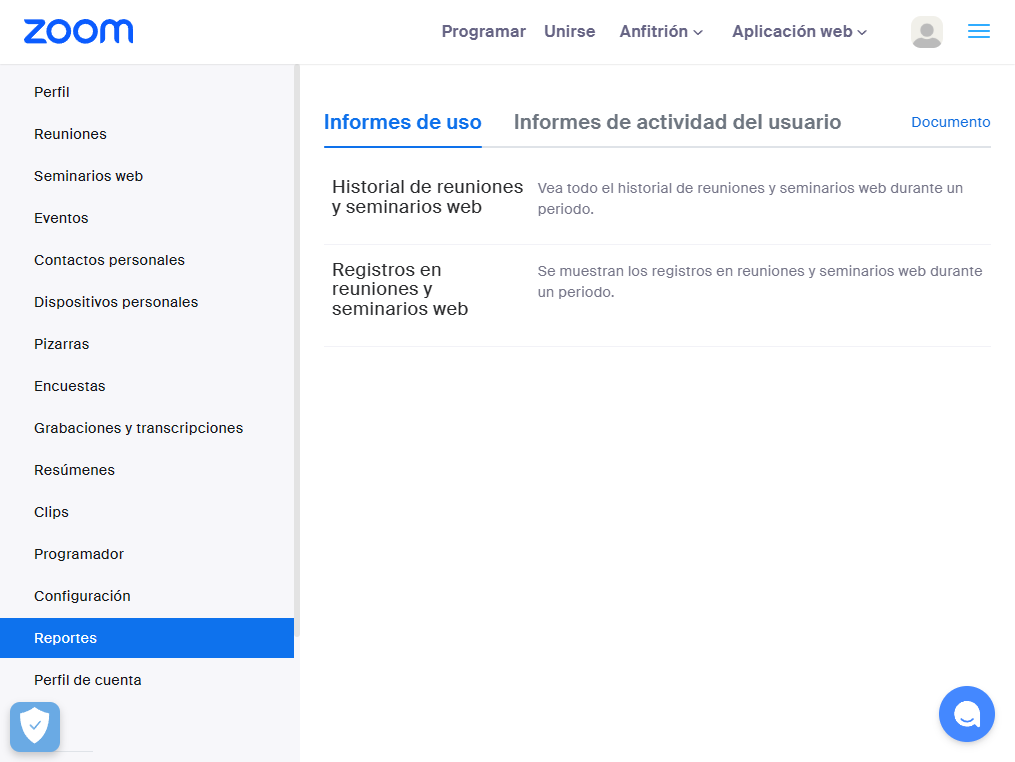
\includegraphics[width=0.8\textwidth]{Sources/zoomReport.png}
                    \caption{Fuente de extracción de los datos (apartado de reportes en \textit{Zoom}) \cite{zoom:reports}.}
                    \label{fig:zoomReport}
                \end{figure}

                Específicamente, para cada mes se tienen dos archivos $\mathsf{.csv}$, donde cada uno contiene su respectiva tabla:
                \begin{enumerate}\label{raw tables dict}
                    \item \textit{registrationMeetings}, que contiene los datos generales de la sesiones programadas (datos previos);
                    \item \textit{usermeeting}, los datos de actividad de las sesiones programadas (datos posteriores y algunos datos redundantes como columnas de \textit{registrationMeetings}, entre otros);
                \end{enumerate}
                
                Se aclara que en los datos de una sesión programada es imposible conocer el número de asistentes, sin embargo en los datos de actividad de las sesiones programadas sí (pues ya sucedió un número de asistentes).
    
                Entonces, si bien no contamos directamente con un único archivo para agrupar la totalidad los datos, mediante un proceso de transformación de los mismos es posible hacerlo. Por ello nos es suficiente contar con los archivos $\mathsf{.csv}$ extraídos.
                
                \begin{figure}[H]
                    \centering
                    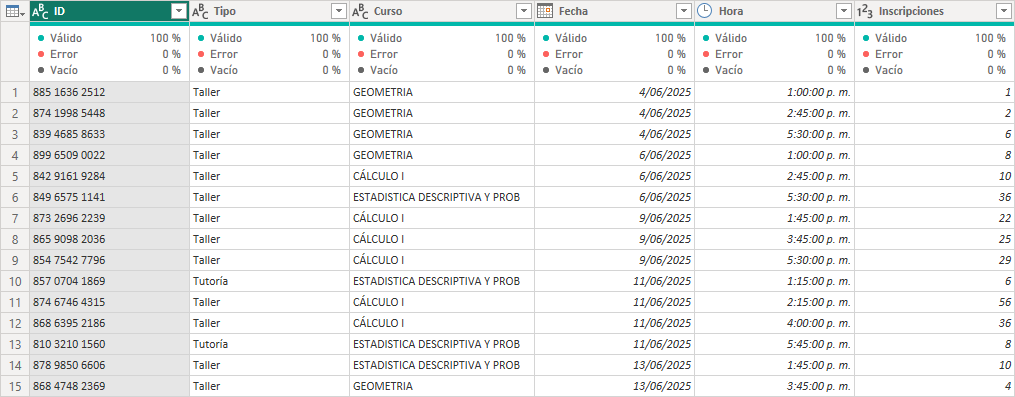
\includegraphics[width=1\textwidth]{Sources/registrationMeetings_Head.png}
                    \caption{Primeras filas de \textit{registrationMeetings}}
                    \label{fig:registrationMeetings_head}
                \end{figure}
                \begin{figure}[H]
                    \centering
                    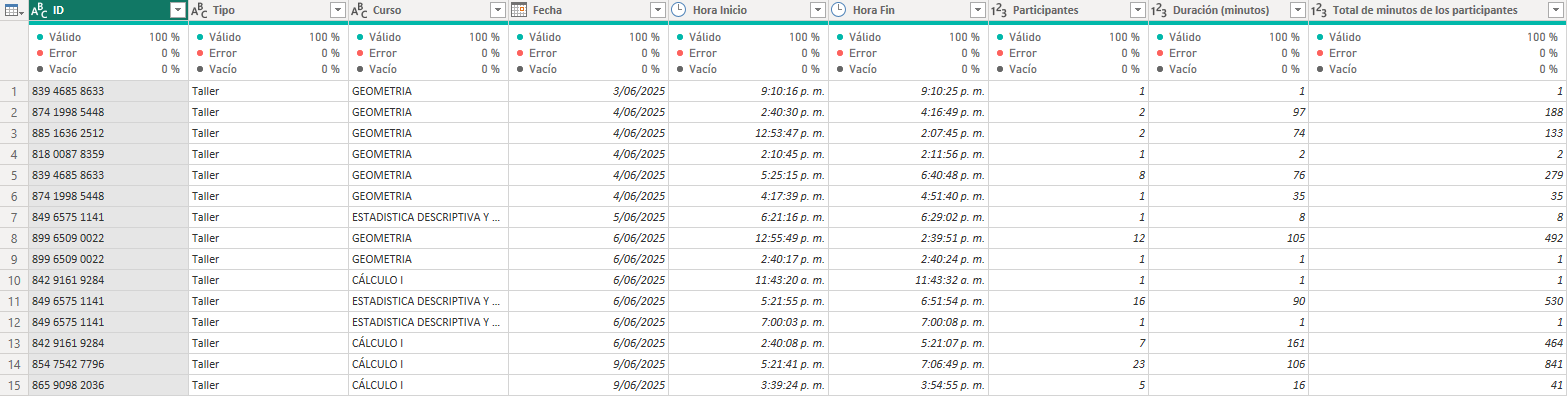
\includegraphics[width=1\textwidth]{Sources/usermeetings_Head.png}
                    \caption{Primeras filas de \textit{usermeeting}}
                    \label{fig:usermeetings_head}
                \end{figure}
            \section{Transformación}
                Hasta este punto se cuenta con dos tipos de tablas: \textit{registrationMeetings} y \textit{usermeeting}. Sin embargo, necesitamos agrupar los datos previos y posteriores para cada sesión existente. Para ello podemos recurrir a cualquier \textit{software} (\textsc{Power BI}, \textsc{PowerQuery}) o lenguaje de programación (\textsc{Python}) que incorpore la operación \textbf{LEFT JOIN}.

                \begin{figure}[H]
                    \centering
                    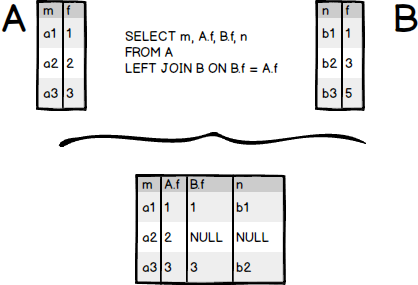
\includegraphics[width=0.4\textwidth]{Sources/SQL-left-join-example.png}
                    \caption{Interpretación gráfica de la operación \textbf{LEFT JOIN} entre dos tablas}
                    \label{fig:SQL-left-join-example}
                \end{figure}
                Esto será posible porque \textit{registrationMeetings} y \textit{usermeeting} cuentan con una columna que contiene el identificador único para cada sesión (\textit{ID} de \textit{Zoom}). Llamaremos a la tabla resultante como \textit{Meetings}.
                
                \begin{figure}[H]
                    \centering
                    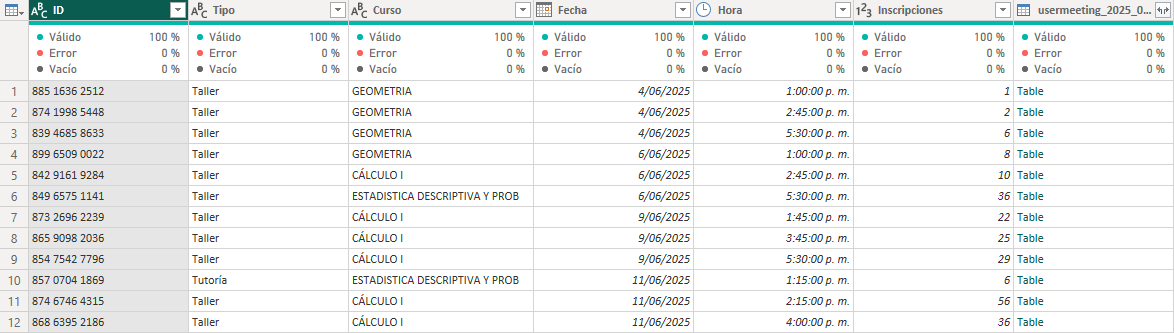
\includegraphics[width=1\textwidth]{Sources/Meetings_Head.png}
                    \caption{Primeras filas de \textit{Meetings}}
                    \label{fig:meetings_head}
                \end{figure}
                \begin{observacion}
                    Para el procedimiento de transformación de las tablas involucradas se utiliza $\textup{\textsc{Power BI}}$ y $\textup{\textsc{PowerQuery}}$.
                \end{observacion}
                
                Ahora, la tarea no es tan sencilla como obtener la tabla \textit{Meetings} y realizar el análisis con la misma, sino que puede verse involucrado un proceso de limpieza (aunque simple) del mismo. Esto es debido a que \textit{Meetings} heredará las demás columnas de \textit{registrationMeetings} y \textit{usermeeting} y, en general, es posible que aparezcan elementos de la tabla con valores \textit{NULL} (lo cual no es favorable para el análisis), filas con \textit{ID} repetido columnas repetidas. Por tanto habrá que realizar a una limpieza de datos en la tabla \textit{Meetings}.

                La mayoría de valores \textit{NULL} aparecen porque \textit{registrationMeetings} contiene datos de sesiones que fueron inicialmente programadas pero posteriormente canceladas y que al operarse mediante \textbf{LEFT JOIN} con \textit{usermeeting} generó datos de actividad inexistentes.
                
                La tabla \textit{Meetings} contiene \textit{ID} repetidos porque en \textit{usermeeting} existen filas con \textit{ID} repetido (como ya se había anticipado en \ref{raw tables dict}). La razón del por qué aparecen estas filas es porque en realidad la tabla \textit{usermeeting} contiene los datos de actividad de las sesiones registradas por \textit{Zoom} con sus correspondientes \textit{ID} e independientemente de la hora programada, es decir, que se puede registrar tanto antes como después de las sesiones programadas que aparecen en \textit{registrationMeetings} (donde todas las filas tienen \textit{ID} único). Por lo tanto, basta que algún estudiante ingrese y salga a una sesión fuera del rango de la hora programada para generar datos de actividad de la misma en \textit{usermeeting}.

                Entonces, el objetivo principal en la limpieza de datos de \textit{Meetings} será:
                \begin{enumerate}\label{pasos transformation}
                    \item Eliminar las filas con datos \textit{NULL} (ya que las sesiones no se realizaron).
                    \item Eliminar las columnas repetidas.
                    \item Eliminar las filas con \textit{ID} repetido.
                \end{enumerate}
                La tabla obtenida de \textit{Meetings} posterior a la limpieza se llamará \textit{MeetingsClean} y esta servirá de base para realizar las transformaciones que sean necesarias.
                \begin{figure}[H]
                    \centering
                    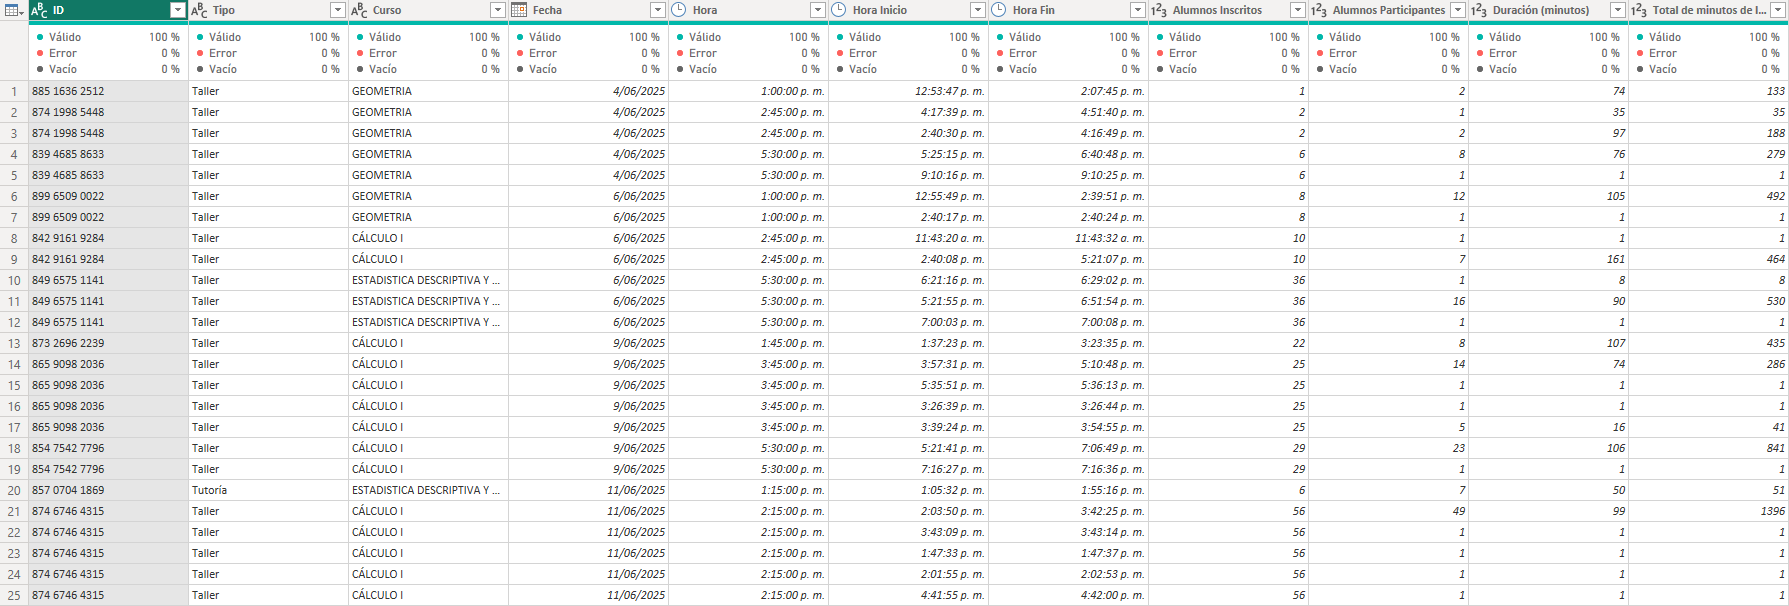
\includegraphics[width=1\textwidth]{Sources/MeetingsClean_Head.png}
                    \caption{Primeras filas de \textit{MeetingsClean}}
                    \label{fig:meetingsclean_head}
                \end{figure}
                Hasta este punto, para obtener los datos (y por tanto los elementos de $\mathcal{S}$) necesarios para el análisis es requerido realizar algunas transformaciones sobre las columnas de \textit{MeetingsClean} sujetas principalmente a separación de caracteres en columnas que contienen texto.

                Finalmente, la tabla resultante de aplicar las transformaciones a las columnas de \textit{MeetingsClean} se llamará \textit{MeetingsCleanInfo}.
                \begin{figure}[H]
                    \centering
                    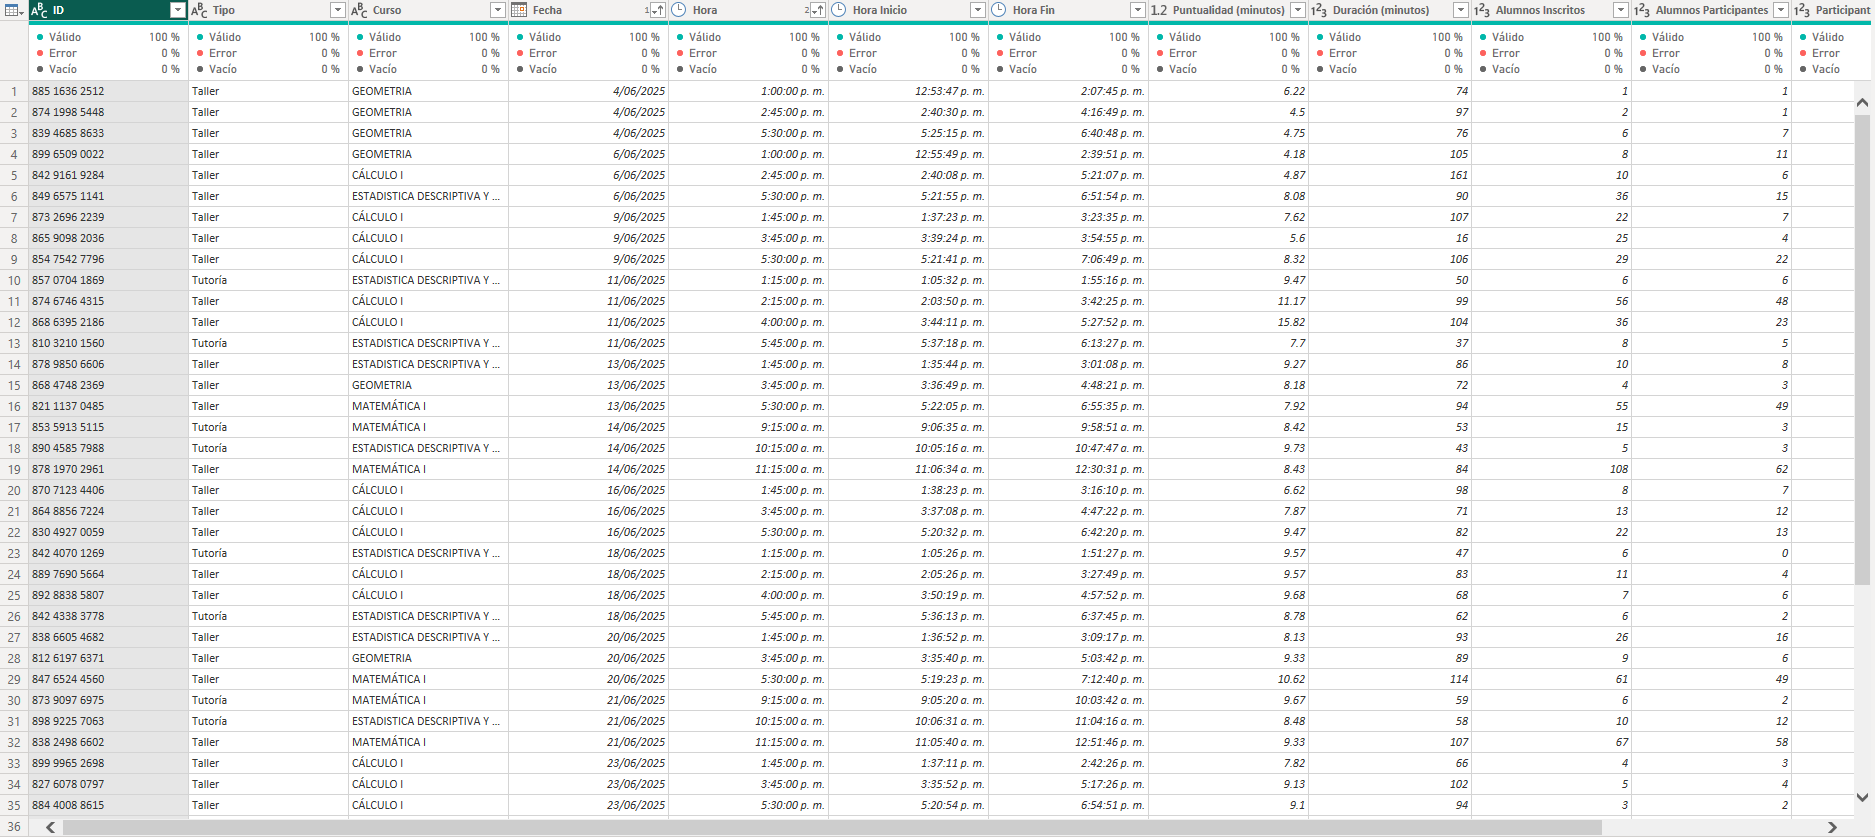
\includegraphics[width=1\textwidth]{Sources/MeetingsCleanInfo_Head.png}
                    \caption{Primeras filas y columnas de \textit{MeetingsCleanInfo}}
                    \label{fig:meetingscleaninfo_head}
                \end{figure}
            \section{Carga}
                Dada la poca complejidad y el poco tamaño de los datos, esta etapa consiste únicamente en la elaboración de gráficos y/o visualizaciones con \textsc{Power BI} a partir de las tablas obtenidas, principalmente \textit{MeetingsCleanInfo}.

            Adelantamos que el tamaño de la tabla \textit{MeetingsCleanInfo} es de 147 filas, y por tanto $\card{\mathcal{S}}=147$, y 12 columnas las cuales son:
            {   \footnotesize
                \begin{multicols}{3}
                    \begin{enumerate}\label{columnas MeetingsCleanInfo}
                        \item \textbf{ID}
                        \item \textbf{Tipo}
                        \item \textbf{Curso}
                        \item \textbf{Fecha}
                        \item \textbf{Hora}
                        \item \textbf{Hora Inicio}
                        \item \textbf{Hora Fin}
                        \item \textbf{Puntualidad (minutos)}
                        \item \textbf{Duración (minutos)}
                        \item \textbf{Alumnos Inscritos}
                        \item \textbf{Alumnos Participantes}
                        \item \textbf{Total de minutos de los participantes}
                    \end{enumerate}
                \end{multicols}
            }
            Asimismo, se presentan los cursos dictados:
            {   \footnotesize
                \begin{multicols}{4}
                    \begin{enumerate}\label{cursos dictados}
                        \item Matemática I
                        \item Matemática II
                        \item Cálculo I
                        \item Cálculo II
                        \item Estadística Descriptiva
                        \item Geometría
                        \item Matemática para Medicina
                    \end{enumerate}
                \end{multicols}
            }
            los cuales son los elementos de $\mathcal{C}$.
        \chapter{Resultados}
            Los resultados obtenidos derivan de un análisis exploratorio de los datos (\textit{EDA}) se utiliza una combinación de uso de \textsc{Power BI} y \textsc{Python}, permitiendo complementar las características y ventajas que cada uno posee. Recordemos que todo el análisis se hace a través de \textit{MeetingsCleanInfo} que contiene los datos de interés (elementos de $\mathcal{S}$).
            
            De hecho, al hacer uso de herramientas que permiten obtener visualizaciones o gráficos (histogramas) a partir de los datos podemos apoyarnos de los mismos para ver qué distribuciones tienen las variables aleatorias involucradas.
            
            Sin embargo, en esta sección solo se presentan los gráficos y tablas sin recurrir a la interpretación de resultados.
             \section{Tipo de sesión}
                Aquí la variable aleatoria analizada es $T_\mathcal{S}$. Esta presenta dos posibles valores: $\text{Taller}$ o $\text{Tutoria}$, por lo que se trata de una variable categórica. Al existir dos posibles valores, se esperaría que la variable aleatoria $T_\mathcal{S}$ sea uniformemente distribuida, es decir,
                \begin{equation}\label{uniforme tipo de sesion}
                    \Prob{T_\mathcal{S}=\text{Taller}}=\Prob{T_\mathcal{S}=\text{Tutoria}}=\frac{1}{2}
                \end{equation}
                De hecho, se puede comprobar ello mediante los datos obtenidos. El siguiente gráfico muestra un gráfico de barras obtenida a partir de \textit{MeetingsCleanInfo} que resume la aproximación obtenida de la distribución de las variables aleatorias $T_\mathcal{S}$.
                \begin{figure}[H]
                    \centering
                    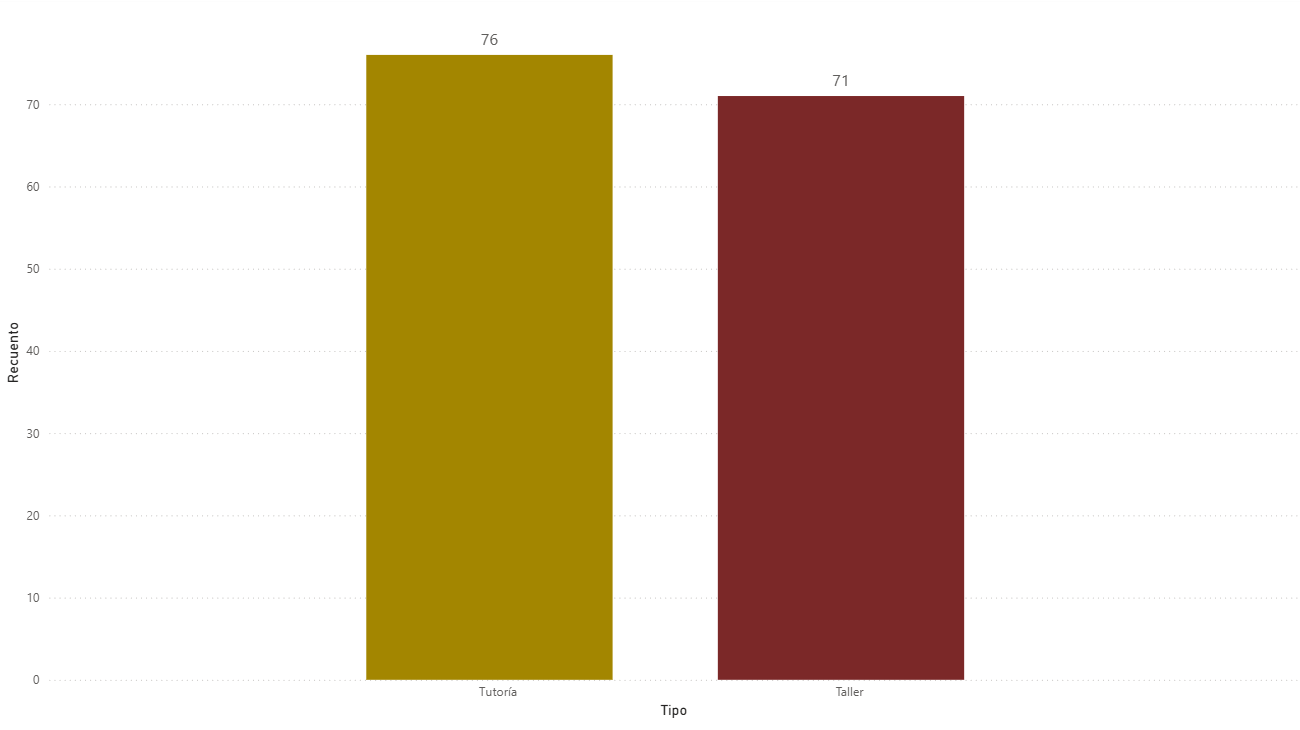
\includegraphics[width=1\textwidth]{Sources/histograma_TipoGlobal.png}
                    \caption{Gráfico de barras del tipo de sesión}
                    \label{fig:histograma_TipoGlobal}
                \end{figure}
                Con ello formamos la tabla
                \begin{table}[H]
                    \centering
                    \begin{tabular}{|c|c|}
                        \hline
                        $t_s$ & $\hat{\Probsymb}_{\mathcal{T}_\mathcal{S}}(t_s)$ \\ \hline
                        Taller & $\frac{71}{147}$ \\ \hline
                        Tutoria & $\frac{76}{147}$ \\ \hline
                    \end{tabular}
                    \caption{Aproximación de la distribución de $T_\mathcal{S}$}
                \end{table}
                Entonces, de acuerdo a lo planteado en \ref{uniforme tipo de sesion} y usando las aproximaciones planteadas en \ref{Otras variables aleatorias Montecarlo} se puede comprobar que la aproximación obtenida de la distribución de $T_\mathcal{S}$ es correcta pues de acuerdo a la gráfica de la Figura \ref{fig:histograma_TipoGlobal}.
                \begin{equation}
                    \hat{\Probsymb}_{\mathcal{T}_\mathcal{S}}(\text{Taller}) = \frac{76}{147} \approx 0.517, \quad \hat{\Probsymb}_{\mathcal{T}_\mathcal{S}}(\text{Tutoria}) = \frac{71}{147} \approx 0.483
                \end{equation}
                Ahora, veamos qué sucede con la distribución de $T_\mathcal{S}$ para cada uno de los cursos, es decir, $T_\mathcal{S}$ dado $C$.
                \begin{figure}[H]
                    \centering
                    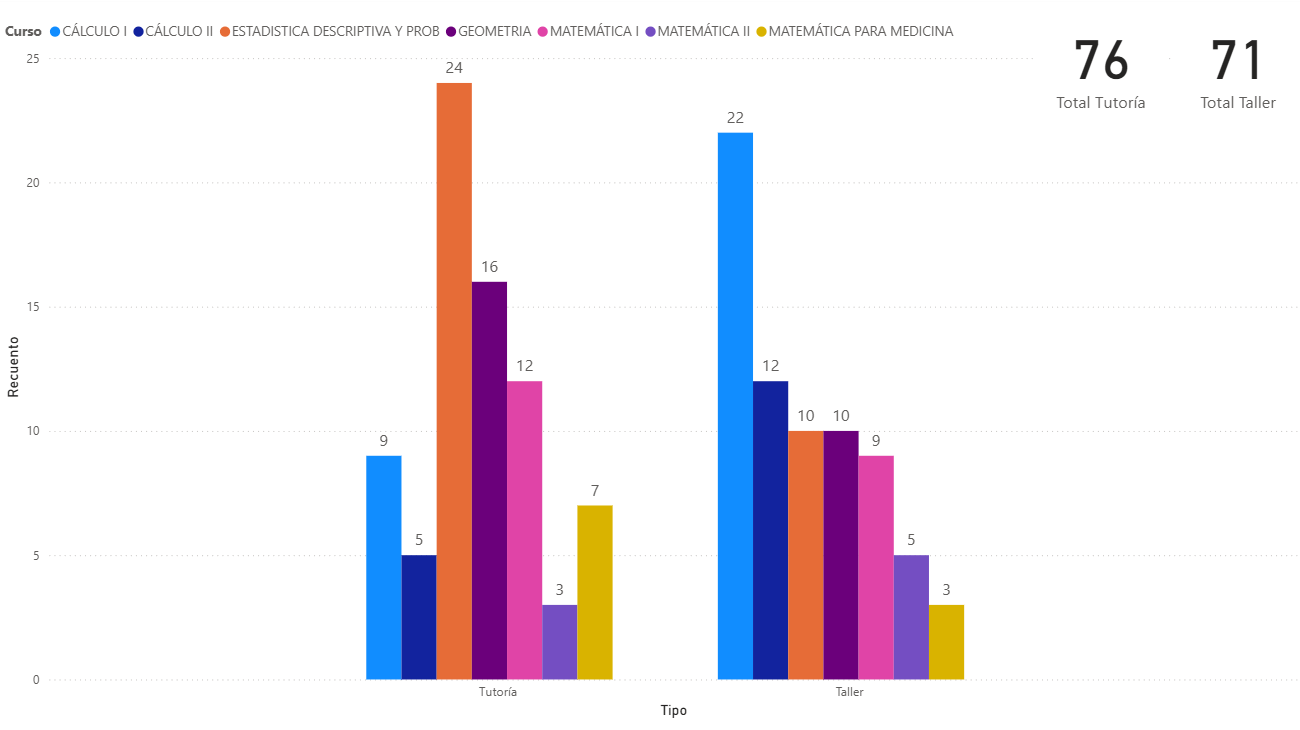
\includegraphics[width=1\textwidth]{Sources/histograma_TipoCurso.png}
                    \caption{Gráfico de barras del tipo de sesión por curso}
                    \label{fig:histograma_TipoCurso}
                \end{figure}
                Dado que tratamos con pocos cursos, es decir $\card{\mathcal{C}}=7$, podemos mostrar en una tabla la aproximación obtenida de la distribución de $T_\mathcal{S}$ dado $C$.
                \begin{table}[H]
                    \centering
                    \begin{tabular}{|c|c|c|c|}
                        \hline
                        \multicolumn{2}{|c|}{\multirow{2}{*}{$\hat{\Probsymb}_{C=c}(T_\mathcal{S}=t_s)$}} & \multicolumn{2}{c|}{$t_s$} \\ \cline{3-4}
                        \multicolumn{2}{|c|}{} & Taller & Tutoría \\ \hline
                        \multirow{7}{*}{$c$} & Matemática I & $\frac{9}{21}$ & $\frac{12}{21}$ \\ \cline{2-4}
                        & Matemática II & $\frac{5}{8}$ & $\frac{3}{8}$  \\ \cline{2-4}
                        & Cálculo I & $\frac{22}{31}$ & $\frac{9}{31}$  \\ \cline{2-4}
                        & Cálculo II & $\frac{12}{17}$ & $\frac{5}{17}$  \\ \cline{2-4}
                        & Estadística Descriptiva & $\frac{10}{34}$ & $\frac{24}{34}$  \\ \cline{2-4}
                        & Geometría & $\frac{10}{26}$ & $\frac{16}{26}$  \\ \cline{2-4}
                        & Matemática para Medicina & $\frac{3}{10}$ & $\frac{7}{10}$   \\ \hline
                    \end{tabular}
                    \caption{Aproximación de la distribución de $T_\mathcal{S}$ dado $C$}
                    \label{tab:distribucion_Ts_C}
                \end{table}
            \section{Cursos dictados}
                Aquí la variable aleatoria analizada es $C$, del cual conocemos los posibles valores que toma ya que conocemos los elementos de $\mathcal{C}$ como se muestra en \ref{cursos dictados}. Por distintos motivos (como demanda) es muy posible que existan cursos con mayor o menor asignación, por lo que no se puede intuir la distribución de $C$. En el siguiente gráfico muestra un gráfico de barras obtenido a partir de \textit{MeetingsCleanInfo} que resume la aproximacion obtenida de la distribución de la variable aleatoria $C$.
                \begin{figure}[H]
                    \centering
                    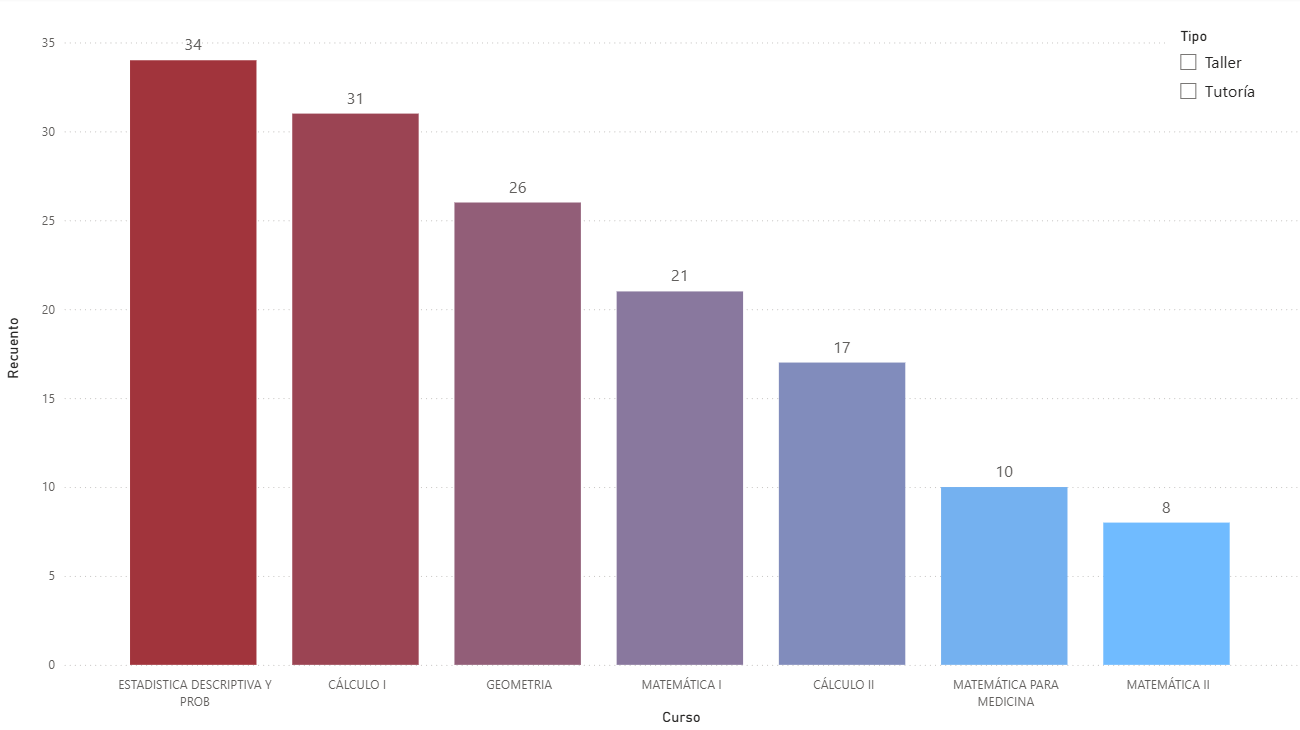
\includegraphics[width=1\textwidth]{Sources/histograma_CursosGlobal.png}
                    \caption{Histograma de los cursos dictados}
                    \label{fig:histograma_CursosGlobal}
                \end{figure}
                Con ello formamos la tabla
                \begin{table}[H]
                    \centering
                    \begin{tabular}{|c|c|}
                        \hline
                        c & $\hat{\Probsymb}_{\mathcal{C}}(c)$ \\ \hline
                        Matemática I & $\frac{21}{147}$ \\ \hline
                        Matemática II & $\frac{8}{147}$ \\ \hline
                        Cálculo I & $\frac{31}{147}$ \\ \hline
                        Cálculo II & $\frac{17}{147}$ \\ \hline
                        Estadística Descriptiva & $\frac{34}{147}$ \\ \hline
                        Geometría & $\frac{26}{147}$ \\ \hline
                        Matemática para Medicina & $\frac{10}{147}$ \\ \hline
                    \end{tabular}
                    \caption{Aproximación de la distribución de $C$}
                \end{table}
                \begin{figure}[H]
                    \centering
                    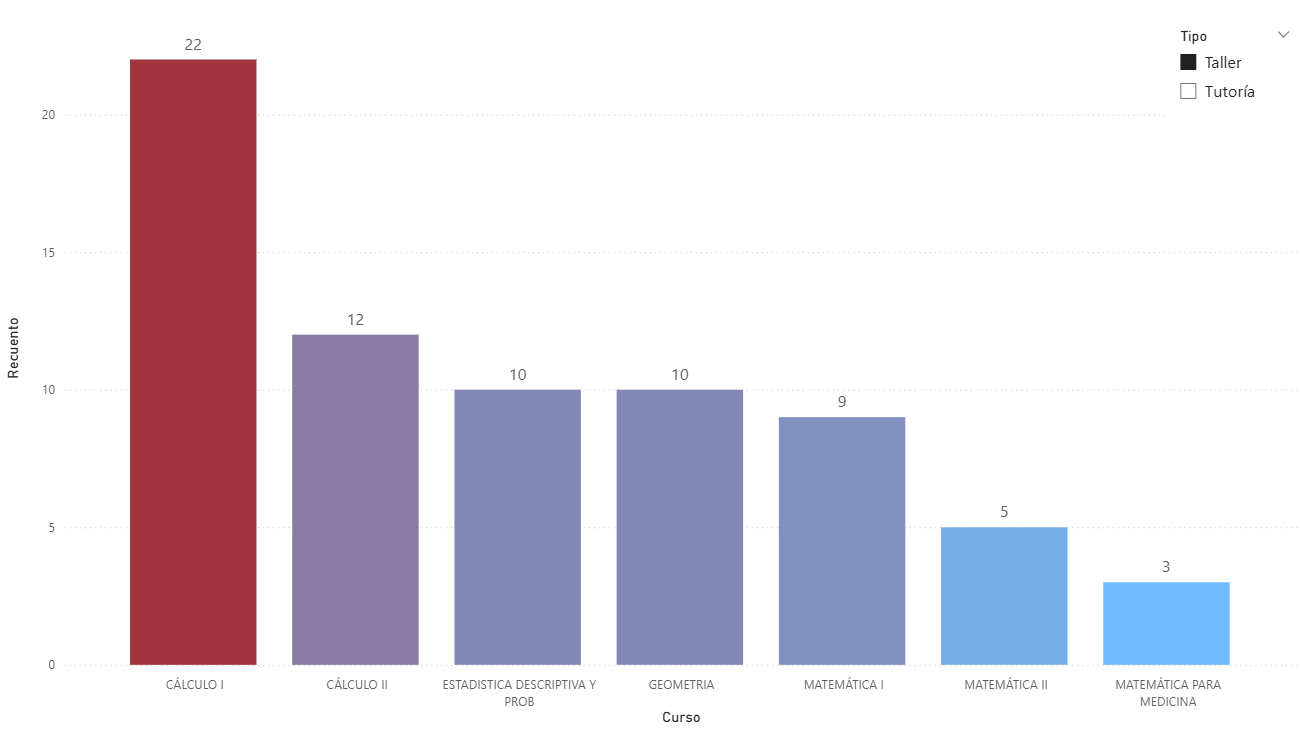
\includegraphics[width=1\textwidth]{Sources/histograma_CursosTaller.png}
                    \caption{Histograma de los cursos dictados en talleres}
                    \label{fig:histograma_CursosTaller}
                \end{figure}
                \begin{figure}[H]
                    \centering
                    \includegraphics[width=1\textwidth]{Sources/histograma_CursosTutoría.png}
                    \caption{Histograma de los cursos dictados en tutorías}
                    \label{fig:histograma_CursosTutoría}
                \end{figure}
                En base a esto último, mostramos la tabla de la aproximación de la distribución de $C$ dado $T_\mathcal{S}$. Se resalta el hecho de que $\card{\mathcal{S}\cap\{s\mid t_s=\text{Taller}\}}=76$ y $\card{\mathcal{S}\cap\{s\mid t_s=\text{Tutoria}\}}=71$ ya que estos valores aparecen en la parte superior de la Figura \ref{fig:histograma_TipoGlobal}.
                \begin{table}[H]
                    \centering                    
                    \begin{tabular}{|c|c|c|c|}
                        \hline
                        \multicolumn{2}{|c|}{\multirow{2}{*}{$\hat{\Probsymb}_{T_\mathcal{S}=t_s}(C=c)$}} & \multicolumn{2}{c|}{$t_s$} \\ \cline{3-4}
                        \multicolumn{2}{|c|}{} & Taller & Tutoría \\ \hline
                        \multirow{7}{*}{$c$} & Matemática I & $\frac{9}{71}$ & $\frac{12}{76}$ \\ \cline{2-4}
                        & Matemática II & $\frac{5}{71}$ & $\frac{3}{76}$  \\ \cline{2-4}
                        & Cálculo I & $\frac{22}{71}$ & $\frac{9}{76}$  \\ \cline{2-4}
                        & Cálculo II & $\frac{12}{71}$ & $\frac{5}{76}$  \\ \cline{2-4}
                        & Estadística Descriptiva & $\frac{10}{71}$ & $\frac{24}{76}$  \\ \cline{2-4}
                        & Geometría & $\frac{10}{71}$ & $\frac{16}{76}$  \\ \cline{2-4}
                        & Matemática para Medicina & $\frac{3}{71}$ & $\frac{7}{76}$  \\ \hline
                    \end{tabular}                    
                    \caption{Aproximación de la distribución de $C$ dado $T_\mathcal{S}$}
                    \label{tab:distribucion_C_Ts}
                \end{table}
            \section{Alumnos inscritos}
                Como sabemos, $\mathcal{I}$ representa la variable aleatoria número de alumnos inscritos en una sesión y mediante \ref{Inscritos-Asistentes Montecarlo} se puede obtener su distribución aproximada, o también mediante \ref{prob total condicional cursos}.
                
                El siguiente gráfico muestra el histograma del número de alumnos inscritos en todas las sesiones, es decir el conteo sobre los valores posibles de $I_s$ para todos los $s\in\mathcal{S}$. Además, como esta variable es de tipo numérica discreta consideramos lo siguiente al realizar la gráfica:
                \begin{itemize}
                    \item No se agrupan los valores de $I_s$ en intervalos.
                    \item Se muestran los estadísticos de la media, desviación estándar, mediana y kurtosis.
                \end{itemize}
                Incluso si los talleres solo permiten un máximo de $100$ alumnos, se observa que existe un único valor dentro de \textit{MeetingsCleanInfo} con $I_s>100$. El fenómeno no podría explicarse a detalle pero se hace el supuesto de que se sucede debido al cómo la plataforma donde los alumnos realizan sus inscripciones regristra los datos. Sin embargo, al tratarse de un único valor este no es tan relevante como para ser excluido de la muestra ya que podemos `ignorar' que el límite de $100$ inscripciones existe.
                \begin{figure}[H]
                    \centering
                    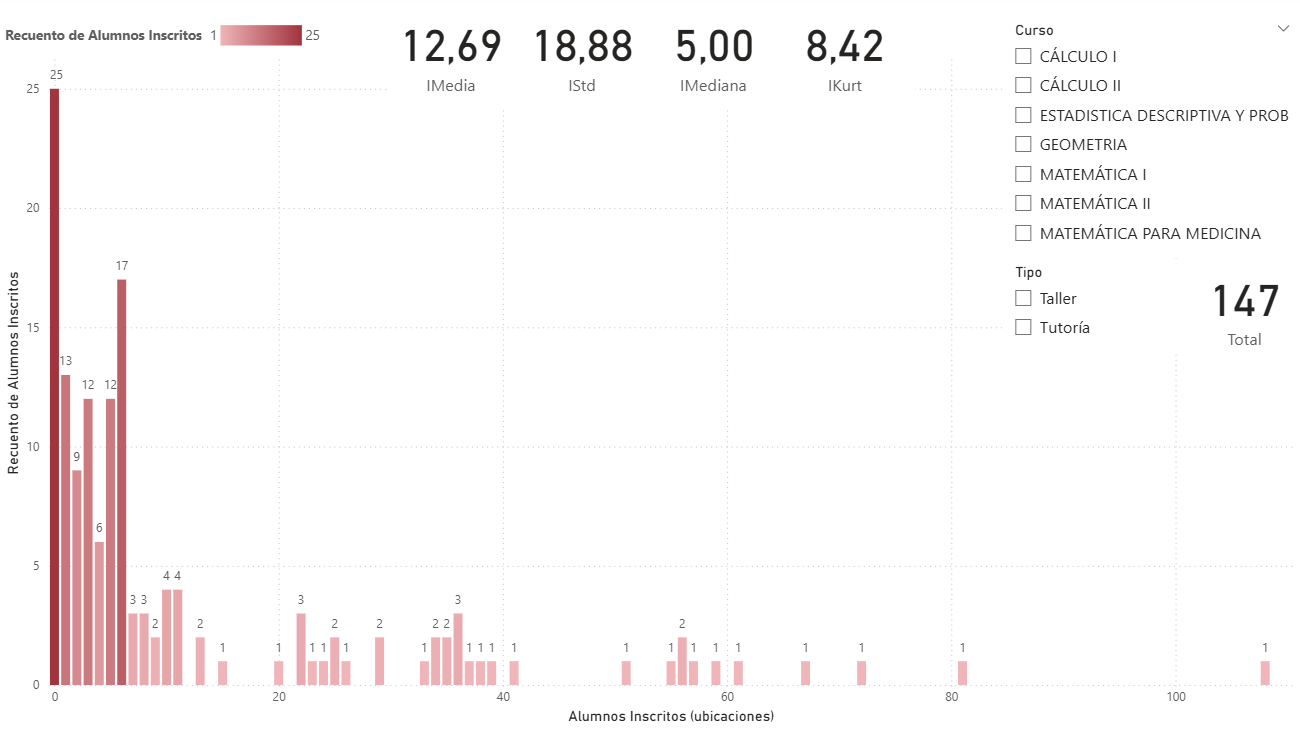
\includegraphics[width=1\textwidth]{Sources/histograma_InscritosGlobal.png}
                    \caption{Histograma de inscritos}
                    \label{fig:histograma_InscritosGlobal}
                \end{figure}
                Lo que es bastante claro de apreciar es que los valores de $I_s$ más frecuentes tienden a ser los que tienen valores más pequeños pero con una alta dispersión. Es decir, el conteo de alumnos inscritos es bastante concentrado en un pequeño rango de valores.
            \section{Alumnos participantes}
                Como sabemos, $\mathcal{A}$ representa la variable aleatoria número de alumnos participantes o asistentes en una sesión y mediante \ref{Inscritos-Asistentes Montecarlo} se puede obtener su distribución aproximada, o también mediante \ref{prob total condicional cursos}.
                
                El siguiente gráfico muestra el histograma del número de alumnos participantes en todas las sesiones, es decir el conteo sobre los valores posibles de $A_s$ para todos los $s\in\mathcal{S}$. Además, como esta variable es de tipo numérica discreta consideramos lo siguiente al realizar la gráfica (al igual que para la Figura \ref{fig:histograma_InscritosGlobal}):
                \begin{itemize}
                    \item No se agrupan los valores de $I_s$ en intervalos.
                    \item Se muestran los estadísticos de la media, desviación estándar, mediana y kurtosis.
                \end{itemize}
                En este caso aparentemente no se observan valores atípicos visibles (a diferencia de lo mostrado en la Figura \ref{fig:histograma_InscritosGlobal}).
                \begin{figure}[H]
                    \centering
                    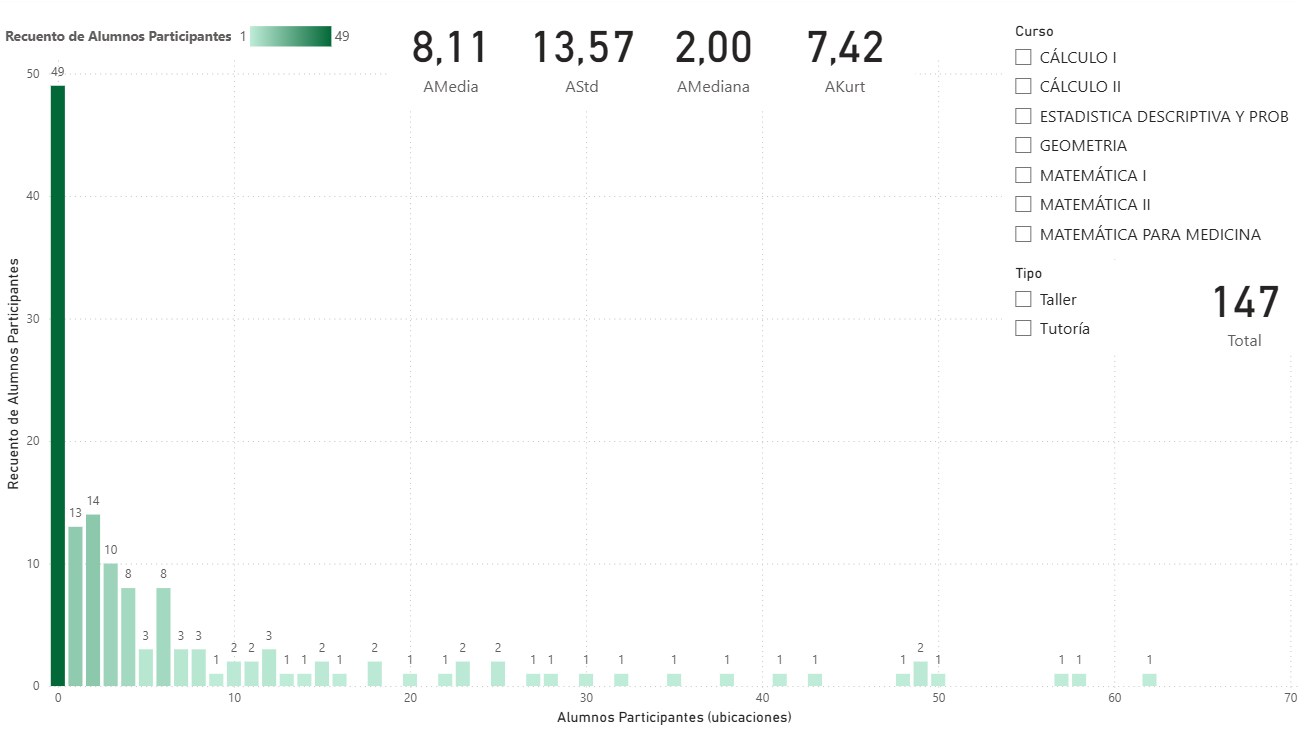
\includegraphics[width=1\textwidth]{Sources/histograma_ParticipantesGlobal.png}
                    \caption{Histograma de participantes}
                    \label{fig:histograma_ParticipantesGlobal}
                \end{figure}
                Lo que sí es apreciable es que la tendencia en la distribución de $A_s$ es bastante similar a la de $I_s$.
            \section{Inscritos-Participantes}
                La relación que tienen $\mathcal{I}$ y $\mathcal{A}$ parece tener algún tipo de dependencia. Como es usual con datos numéricos, se puede analizar los coeficientes de correlación (Pearson) entre los mismos. Mediante el uso de librerías de \textsc{Python} se puede obtener la matriz de correlación (Pearson) asociada.
                \begin{figure}[H]
                    \centering
                    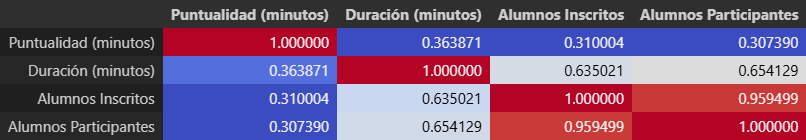
\includegraphics[width=0.7\textwidth]{Sources/corrmatrix_NumericalFeatures.png}
                    \caption{Correlación de las variables numéricas}
                \end{figure}
                Lo que muestra la matriz de correlación permitiría explicar el por qué de la similitud entre los histogramas de las variables aleatorias $I$ e $A$. El coeficiente de correlación entre ambas variables es muy próxima a $1$ lo que indica una alta correlación positiva, y además es el coeficiente de correlación más alto de todas las variables numéricas.
                
                En el siguiente gráfico se muestra la dispersión de $(\mathcal{I}_s,\mathcal{A}_s)$ para $s\in\mathcal{S}$, es decir, los pares inscritos-participantes obtenidos a partir de \textit{MeetingsCleanInfo}.
                \begin{figure}[H]
                    \centering
                    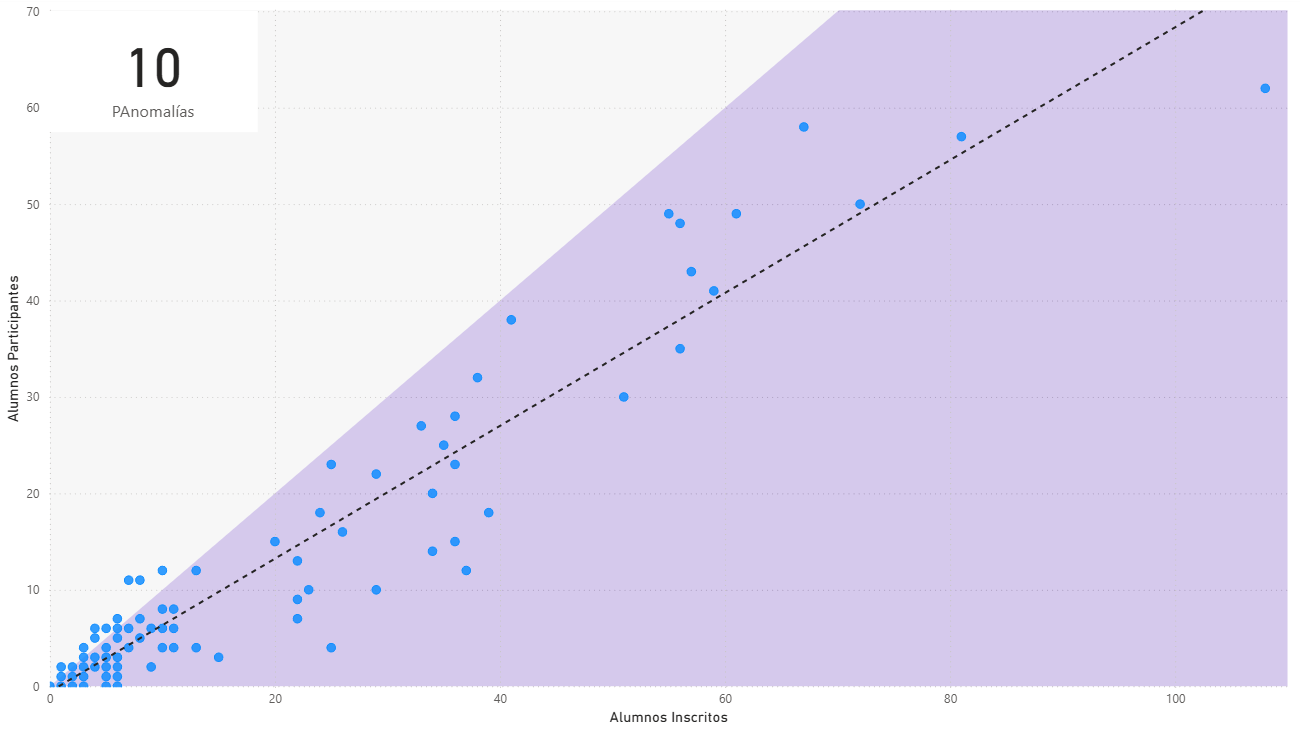
\includegraphics[width=1\textwidth]{Sources/dispersion_InscritosParticipantes.png}
                    \caption{Dispersión de $(\mathcal{I}_s,\mathcal{A}_s)$ para cada $s\in\mathcal{S}$}
                    \label{fig:dispersion_InscritosParticipantes}
                \end{figure}
                La región sombreada representa la región de pares inscritos-participantes que tiene un comportamiento `regular', es decir, que $\mathcal{I}_s\geq \mathcal{A}_s$ (ya que no es posible que alguien asista sin estar previamente inscrito, en teoría). En base a ello, sólo se contabilizan $10$ pares que no presentan el comportamiento `regular' y los consideramos como atípicos o `anómalos'.

                Por otro lado, dado que la correlación lineal entre $I$ y $A$ es bastante alta, podemos usar la regresión lineal para obtener una aproximación de la distribución de $A$ dado $I$. En la Figura \ref{fig:dispersion_InscritosParticipantes} se muestra la recta de regresión lineal en base a los datos obtenidos y aparece en forma de línea punteada. Sin embargo, como este gráfico fue elaborado en \textsc{Power BI}, este no se muestra con una ecuación explícita pero podemos encontrarla utilizando las librerías existentes en \textsc{Python}.

                Así, la ecuación de la recta de regresión lineal obtenida se muestran en el siguiente gráfico.
                \begin{figure}[H]
                    \centering
                    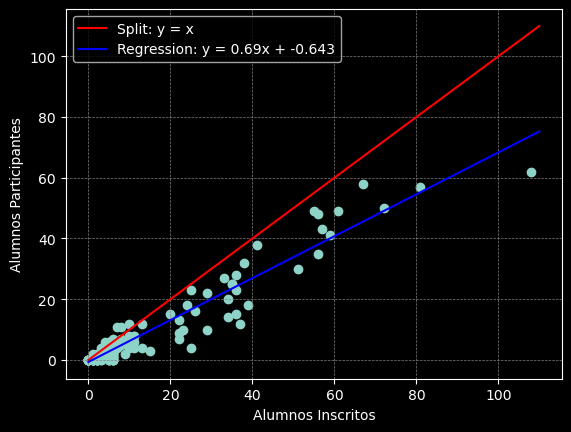
\includegraphics[width=0.7\textwidth]{Sources/linearregression_InscritosParticipantes.png}
                    \caption{Regresión lineal de la variable aleatoria $\mathcal{I},\mathcal{A}$}
                \end{figure}
                Entonces para $x\in\Real^+\cap\Integer$ representando el número de alumnos inscritos en una sesión (que es conocido antes de una sesión) tendríamos que $y=0.69x-0.643$, con un redondeo adecuado, representaría el número estimado de asistentes en la sesión.

                Si bien esto muestra el comportamiento global del par inscritos-participantes se desconoce el comportamiento según el curso.

                Por otro lado, si trabajamos en base al supuesto $A\approx0.69I-0.643+\varepsilon_I$ con $\varepsilon_I\sim\mathcal{N}(0,\sigma_I^2)$ entonces
                \begin{equation*}
                    \EV{A\mid I=n}\approx 0.69n-0.643
                \end{equation*}
                y deberíamos ser capaces de verificar que $A-0.69I+0.643\sim\varepsilon_I\sim\mathcal{N}(0,\sigma_I^2)$ mediante el contraste de hipótesis.
            \section{Duración de sesiones}
                La columna \textbf{Duración (minutos)} no se encuentra originalmente en \textit{MeetingsClean} sino que se añade a la misma apareciendo en \textit{MeetingsCleanInfo}. Esta columna contiene la diferencia (en minutos) de la hora fin la hora de inicio de la sesión en su correspondiente fila, por lo que podemos decir que 
                \begin{equation*}
                    \textup{\textbf{Duración}}:=\textup{\textbf{Hora Fin}}-\textup{\textbf{Hora Inicio}}
                \end{equation*}
                
                Además, como esta variable es de tipo numérica continua consideramos lo siguiente al realizar la gráficas:
                \begin{itemize}
                    \item Se agrupan los valores de $I_s$ en intervalos de $8\,\textup{min}$.
                    \item Se muestran los estadísticos de la media, desviación estándar, mediana y kurtosis.
                \end{itemize}
                El motivo de agrupar en intervalos de $8\,\textup{min}$ es porque si buscaramos partir en $9$ subintervalos los intervalos $[0;45]$ y $[0;90]$, los intervalos tendrían longitud $5\,\textup{min}$ y $10\,\textup{min}$ respectivamente, por lo que para evitar el tener que utilizar intervalos de longitud diferentes se toman intervalos que resulten del promedio aproximado de los mismos que es $7.5\,\textup{min}\approx8\,\textup{min}$.

                En el comportamiento global de esta variable podría no ser apreciable algún comportamiento en particular.
                \begin{figure}[H]
                    \centering
                    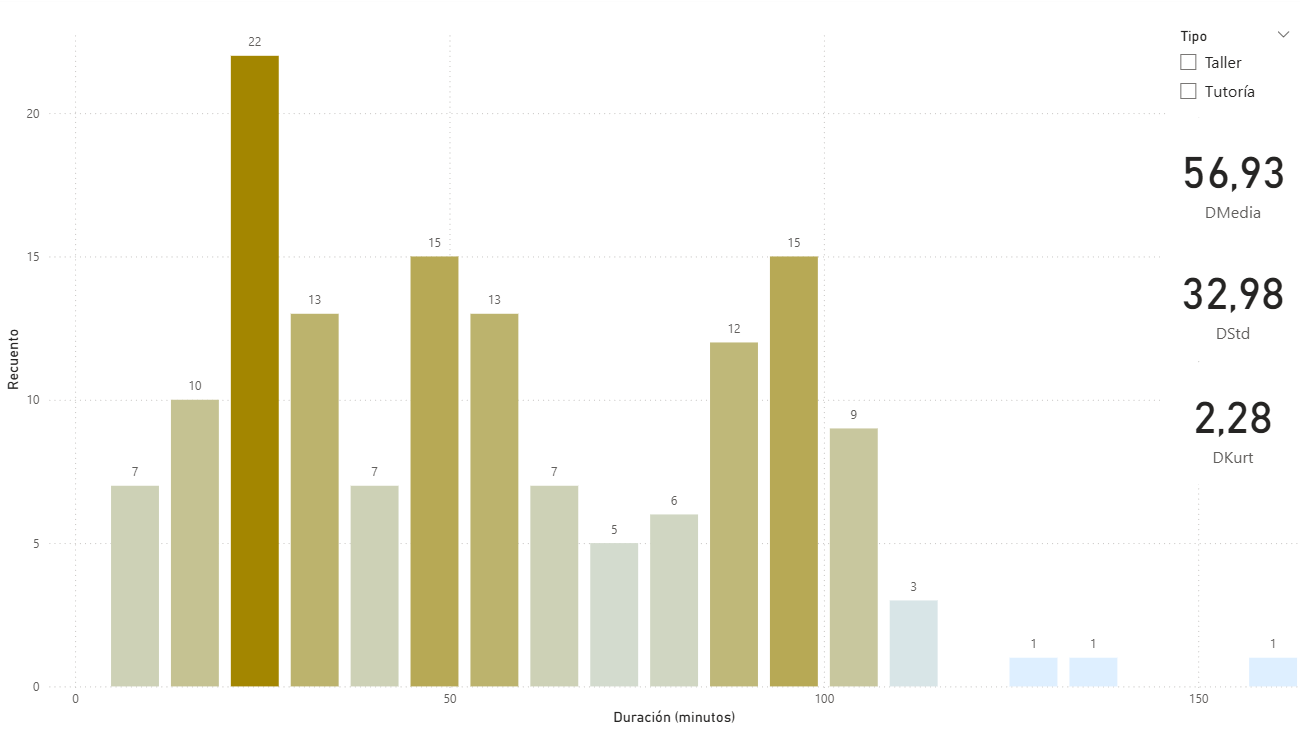
\includegraphics[width=1\textwidth]{Sources/histograma_DuracionGlobal.png}
                    \caption{Histograma de la duración de las sesiones}
                \end{figure}
                Sin embargo, como ya se ha mencionado, según el tipo de sesión la duración máxima establecida de la misma es diferente. Es decir, $90\,\textup{min}$ para los talleres y $45\,\textup{min}$ para las tutorías. Por lo tanto, se espera que la mayor parte de los valores registrados en la columna \textbf{Duración (minutos)} estén mayoritariamente concentrados en $90$ y $45$ para los talleres y tutorías, respectivamente.
                \begin{figure}[H]
                    \centering
                    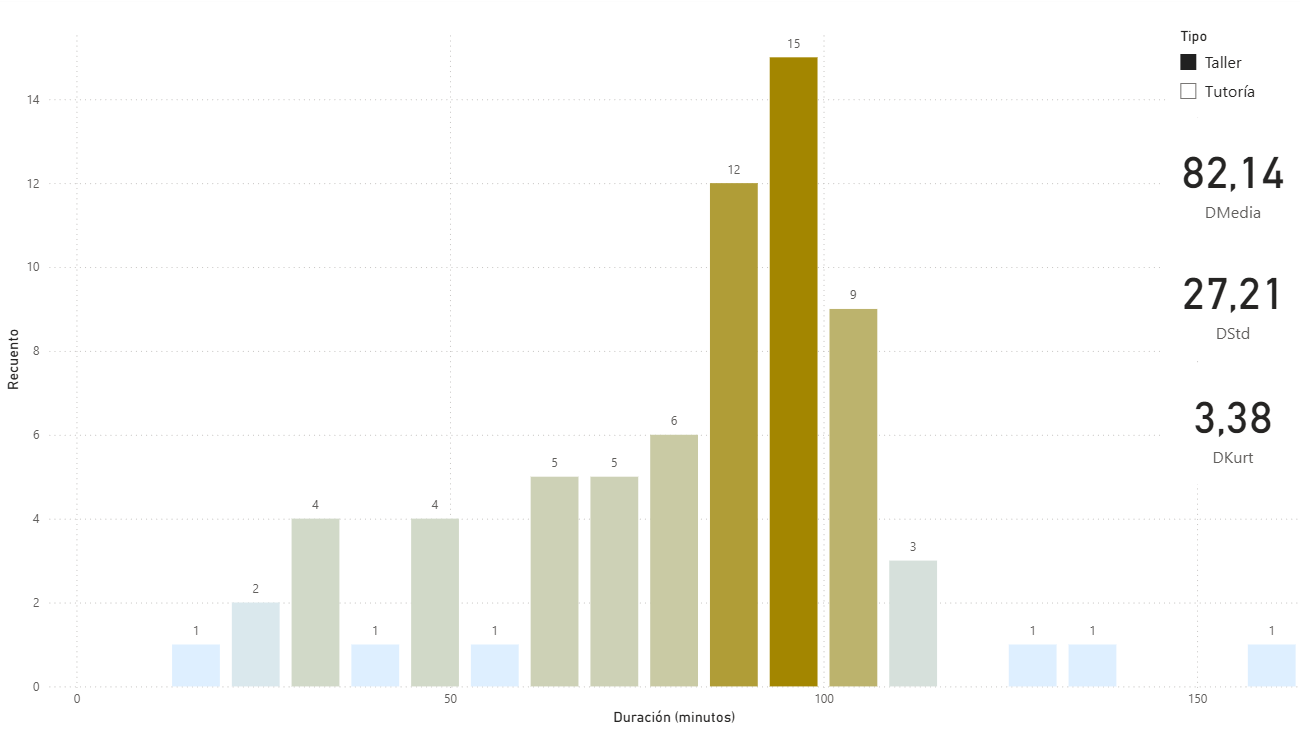
\includegraphics[width=1\textwidth]{Sources/histograma_DuracionTaller.png}
                    \caption{Histograma de la duración de las sesiones en talleres}
                \end{figure}
                \begin{figure}[H]
                    \centering
                    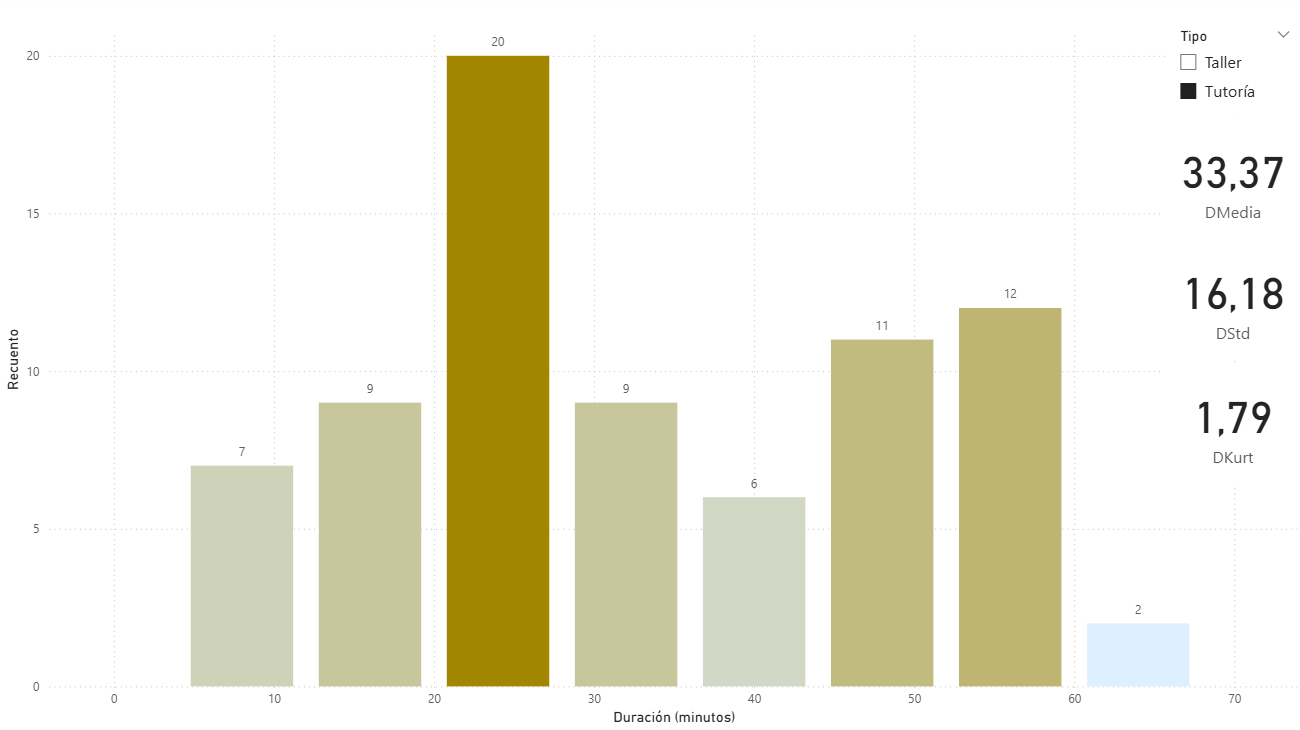
\includegraphics[width=1\textwidth]{Sources/histograma_DuracionTutoria.png}
                    \caption{Histograma de la duración de las sesiones en tutorías}
                \end{figure}
            \section{Puntualidad}
                La columna \textbf{Puntualidad (minutos)}, o de forma simplificada \textbf{Puntualidad}, no se encuentra originalmente en \textit{MeetingsClean} sino que se añade a la misma apareciendo en \textit{MeetingsCleanInfo}. Esta columna contiene la diferencia (en minutos) de la hora programada y la hora de inicio de la sesión en su correspondiente fila, por lo que podemos decir que 
                \begin{equation*}
                    \textup{\textbf{Puntualidad}}:=\textup{\textbf{Hora}}-\textup{\textbf{Hora Inicio}}
                \end{equation*}
                Además, como esta variable es de tipo numérica continua consideramos lo siguiente al realizar la gráficas:
                \begin{itemize}
                    \item Se agrupan los valores de $\textup{\textbf{Puntualidad}}$ en intervalos de $1\,\textup{min}$.
                    \item Se muestran los estadísticos de la media, desviación estándar, mediana y kurtosis.
                \end{itemize}
                
                Dado que el reglamento de la \textit{Universidad Tecnológica del Perú} indica que, tanto para talleres como para tutorías, la hora de ingreso a la sesión debe ser entre $5$ y $10$ minutos antes de la hora programada, entonces se esperaría que los valores registrados en la columna \textbf{Puntualidad (minutos)} se encuentren mayoritariamente concentrados en el intervalo $\mathopen[5;10\mathclose]$.
                
                Sin embargo, también debemos tener en cuenta que podrían presentarse valores atípicos, pues como ya se mencionó \textit{Zoom} registra que una sesión ha sido iniciada si es que existe algún integrante en la sesión e independiente de si se trata del anfitrión (mi persona) o no.
                \begin{figure}[H]
                    \centering
                    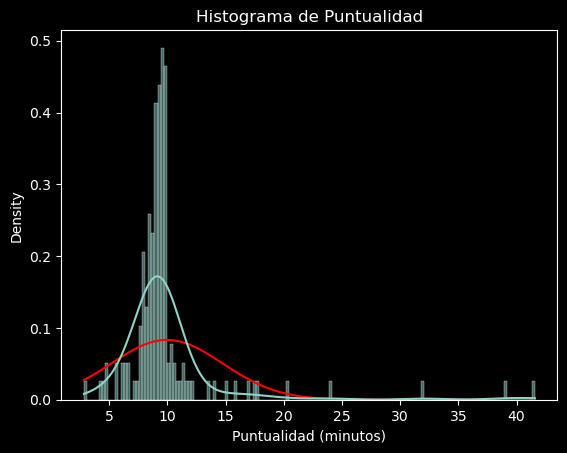
\includegraphics[width=0.7\textwidth]{Sources/histogram_Puntualidad.png}
                    \caption{Histograma de la puntualidad (\textsc{Python})}
                \end{figure}
                En efecto, los valores atípicos se aparecen y estos son los valores de \textbf{Puntualidad} más altos. Esto podría explicarse mediante el hecho de que algún estudiante ingresó a la sesión minutos muy antes de la hora programada y permaneció hasta la hora en que el anfitrión ingresó.
                \begin{figure}[H]
                    \centering
                    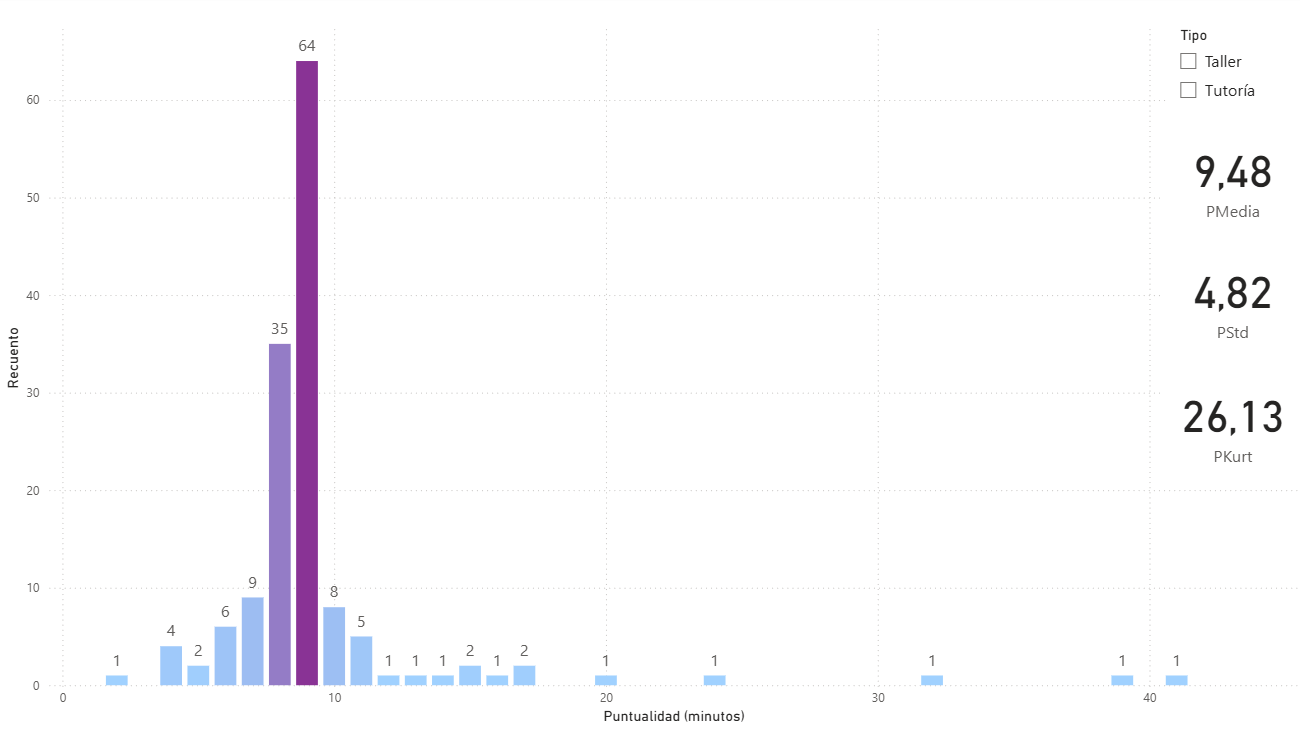
\includegraphics[width=1\textwidth]{Sources/histograma_PuntualidadGlobal.png}
                    \caption{Histograma de la puntualidad (\textsc{Power BI})}
                \end{figure}
                El comportamiento global es muy similar al observado al comportamiento en talleres y tutorías.
                \begin{figure}[H]
                    \centering
                    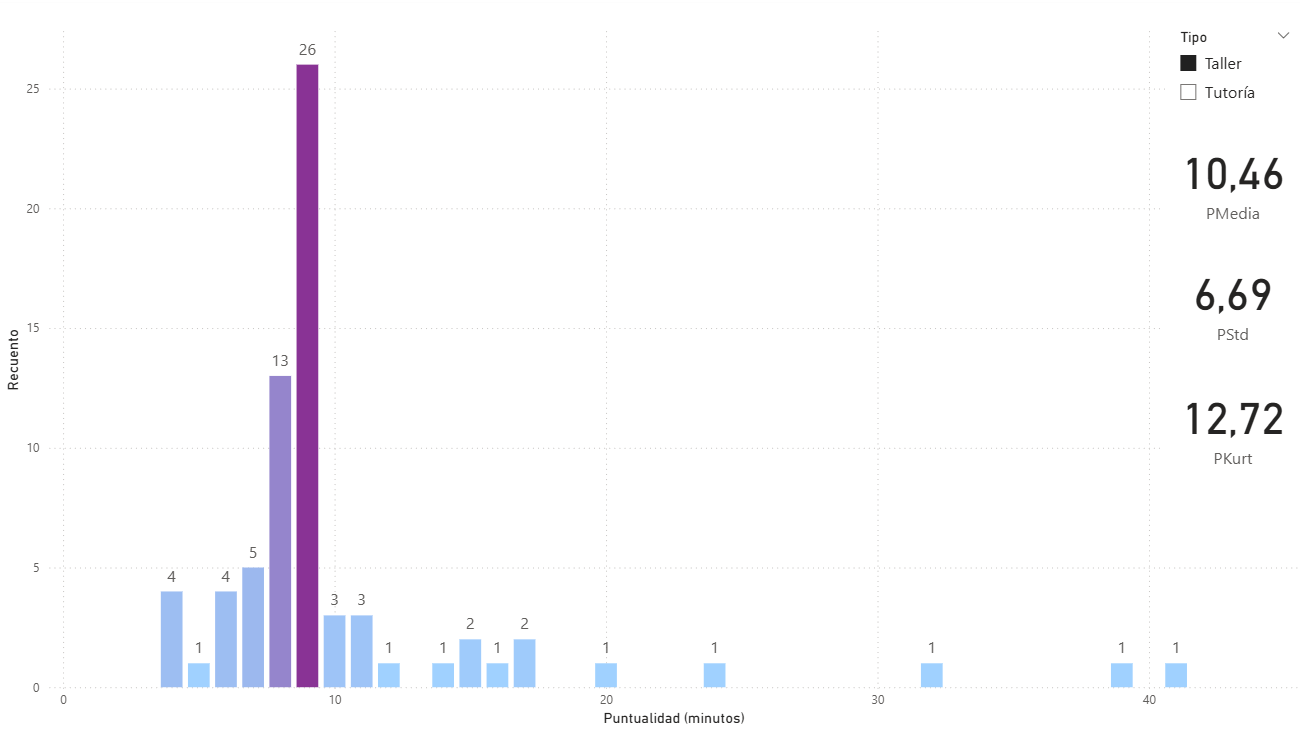
\includegraphics[width=1\textwidth]{Sources/histograma_PuntualidadTaller.png}
                    \caption{Histograma de la puntualidad en talleres}
                \end{figure}
                \begin{figure}[H]
                    \centering
                    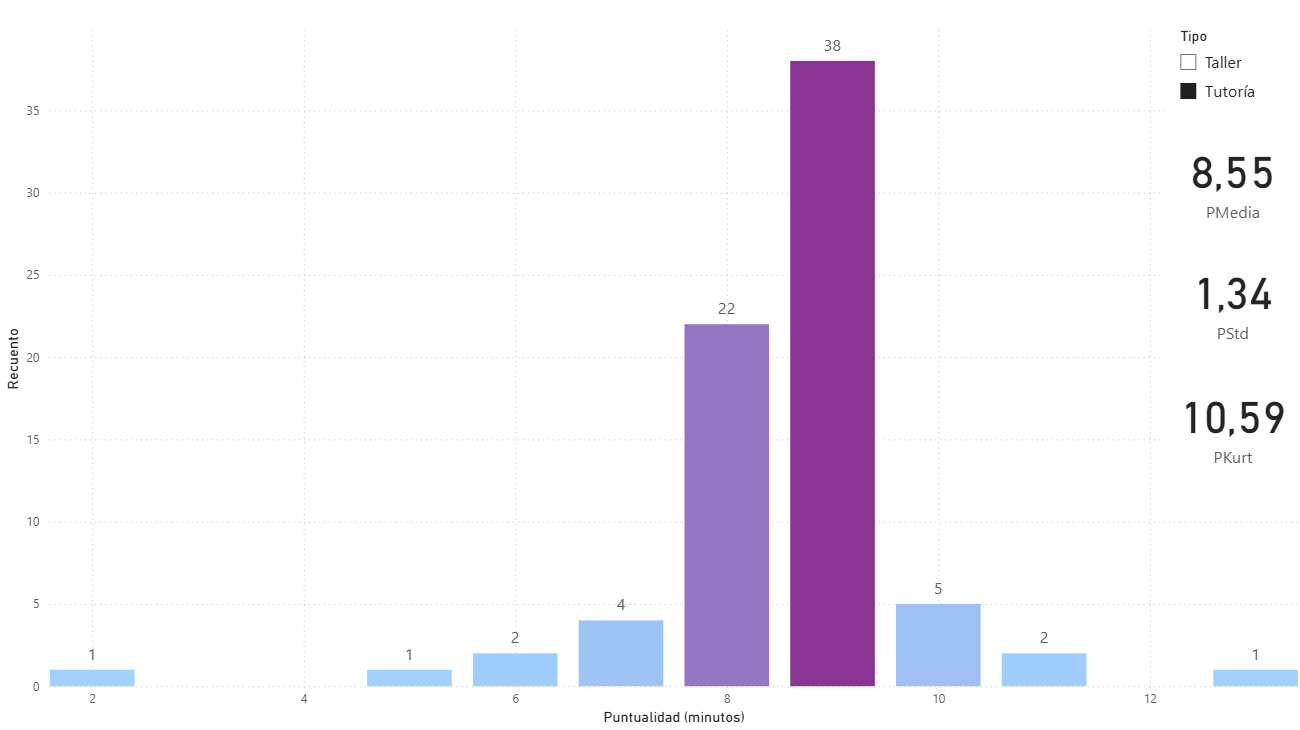
\includegraphics[width=1\textwidth]{Sources/histograma_PuntualidadTutoria.png}
                    \caption{Histograma de la puntualidad en tutorías}
                \end{figure}
                Esto tiene sentido, pues, debido a que la puntualidad es indistinta al tipo de sesión.
    \chapter{Resultados}        
        \section{Por curso}
            \subsection{Matemática I}
            \subsection{Matemática II}
            \subsection{Cálculo I}
            \subsection{Cálculo II}
            \subsection{Estadística Descriptiva}
            \subsection{Geometría}
        \section{Por tipo}
            \subsection{Talleres}
            \subsection{Tutorías}
        \section{Por fecha y hora}
    \chapter{Discusión}
        
    \chapter{Conclusiones}
        Distribución del número de inscritos (Por curso y global: el número global es la suma de los números por curso (variables aleatorias))
        \begin{enumerate}
            \item La distribución de la duración de las sesiones es muy diferente en talleres y tutorías.
            \item La distribución de la puntualidad de las sesiones es muy diferente en talleres y tutorías.
            \item La distribución de la cantidad de inscritos es muy diferente en talleres y tutorías.
            \item El número de asistentes presenta una correlación lineal positiva fuerte con el número de inscritos.
        \end{enumerate}
    \chapter{Anexos}
        \begin{definicion}[Función indicatriz]
            Sea $A$ un subconjunto de un conjunto $X$, definimos la función indicatriz de $A$ sobre $X$ como $\mathds{1}_A:X\longrightarrow\{0,1\}$ con
            \begin{equation*}
                \mathds{1}_A (x)=\left\{\begin{array}{cl}
                    1&,\enspace x\in A  \\
                    0&,\enspace x \in A^\setcomplement
                \end{array}\right.
            \end{equation*}
        \end{definicion}
        \section{Probabilidad}
            \begin{definicion}[Probabilidad condicional]
                Sean $A$ y $B$ eventos de un espacio de probabilidad $(\Omega,\mathcal{F},\Probsymb)$. La probabilidad de $A$ dado $B$ se define como
                \begin{equation}
                    \Probsymb(A \mid B) :=\dfrac{\Probsymb(A\cap B)}{\Probsymb(B)}
                \end{equation}
            \end{definicion}
            \begin{definicion}[Partición]
                Decimos que los $A_{1}, A_{2}, \dots, A_{n}\subset A$ forman una partición de $A$ si los $A_i$ son exhaustivos y mutuamente excluyentes.
            \end{definicion}
            \begin{definicion}[Partición de un espacio de probabilidad]
                Decimos que los $A_{1}, A_{2}, \dots, A_{n}\subset A$ forman una partición de un espacio de probabilidad $(\Omega,\mathcal{F},\Probsymb)$ si $A_i\in\mathcal{F},\enspace i =1,\ldots,n$ y forman una partición de $\Omega$.
            \end{definicion}
            \begin{teorema}[Bayes]\label{T. bayes}
                Sea $A_{1}, A_{2}, \dots, A_{n}$ una partición del espacio de probabilidad $(\Omega,\mathcal{F},\Probsymb)$ tales que $\Probsymb(A_i) > 0,\enspace i=1,\ldots,n$. Sea $B$ un evento arbitrario de $(\Omega,\mathcal{F},\Probsymb)$, entonces
                \begin{equation}
                    \Probsymb(A_i \mid B) = \frac{\Probsymb(B \mid A_i)\, \Probsymb(A_i)}{\Probsymb(B)}
                \end{equation}
            \end{teorema}
            \begin{teorema}[Probabilidad total]
                Bajo las mismas condiciones del Teorema \ref{T. bayes},
                \begin{equation}
                    \Probsymb(B) = \sum_{i=1}^n \Probsymb(B \mid A_i)\Probsymb(A_i)
                \end{equation}
                Además se obtiene la \textbf{fórmula de Bayes}
                \begin{equation}
                    \Probsymb(A_i \mid B) = \frac{\Probsymb(B \mid A_i)\, \Probsymb(A_i)}{\sum_{i=1}^n \Probsymb(B \mid A_i)\Probsymb(A_i)}
                \end{equation}
            \end{teorema}
            \begin{definicion}[Distribución normal]
                Una variable aleatoria \(X\) es normalmente distribuida con media \(\mu\) y varianza \(\sigma^{2}\) si su densidad es 
                \begin{equation}
                    f(x) = \frac{1}{\sqrt{2\pi\sigma^{2}}}\exp{-\frac{(x-\mu)^{2}}{2\sigma^{2}}}
                \end{equation}
                y en tal caso denotamos \(X \sim \mathcal{N}(\mu,\sigma^{2})\). Además, si $\mu=0$ y $\sigma=1$ se dice que \(X\) es normalmente distribuida.
            \end{definicion}
            \begin{teorema}[Ley débil de los grandes números]\label{large numbers weak}
                Sea  $X_{1}, X_{2}, X_{3}, \dots$ una sucesión de variables aleatorias independientes e idénticamente distribuidas con valor esperado 
                \(\mu\) y varianza \(\sigma^{2}\), entonces el promedio
                \[
                \overline{X}_{n} = \frac{X_{1} + \cdots + X_{n}}{n}
                = \frac{1}{n} \sum_{i=1}^{n} X_{i}
                \]
                converge en probabilidad a \(\mu\). En otras palabras, para cualquier 
                \(\varepsilon>0\) se cumple que
                \[
                \lim_{n \to \infty} \, P\!\left( \left|\overline{X}_{n} - \mu \right| < \varepsilon \right) = 1.
                \]
            \end{teorema}
            \begin{teorema}[Ley fuerte de los grandes números]\label{large numbers strong}
                Sea  $X_{1}, X_{2}, X_{3}, \dots$ una sucesión de variables aleatorias independientes e idénticamente distribuidas que cumplen 
                \(\EV{X_{i}}< \infty\) y tienen valor esperado 
                \(\EV{X_{i}}= \mu\), entonces
                \begin{equation*}
                    \Prob{ \lim_{n \to \infty} \overline{X}_{n} = \mu}= 1,
                \end{equation*}
                es decir, el promedio de las variables aleatorias converge a \(\mu\) casi seguramente. 
            \end{teorema}

        \section{Métricas estadísticas}
            \begin{definicion}[Matriz de covarianza]
                Sea $X=(X_1,X_2,\dots,X_n)$ una variable aleatoria en $\mathbb{R}^n$ con $X_i$ de varianza y media finitas. La \textbf{matriz de covarianza} de $X$ se define como 
                \begin{equation*}
                    K_{XX} := \Var{X} := \textup{cov}(X,X) := \EV{(X-\EV{X})(X-\EV{X})^T}
                \end{equation*}
            \end{definicion}
            \begin{definicion}[Estimador (estadístico)]
                Es una función generada a partir de los datos de una muestra que se usa para estimar algún parámetro desconocido de la población. Cuando el estimador toma un valor en particular en base a los datos de una muestra, se llama \textbf{estimador puntual}.
            \end{definicion}

            \begin{definicion}[Sesgo de un estimador]
                Sea $\hat{\theta}$ un estimador de un parámetro $\theta$. Entonces el sesgo o \textit{bias} de $\hat{\theta}$ se define como
                \begin{equation*}
                    B(\hat{\theta}) = \EV{\hat{\theta}} - \theta
                \end{equation*}
                Si $B(\hat{\theta}) = 0$, entonces $\hat{\theta}$ decimos que es un \textbf{estimador insesgado}.
            \end{definicion}

            \begin{definicion}[Consistencia de un estimador]
                Sea $\hat{\theta}_n$ un estimador de un parámetro $\theta$ determinado por una muestra de tamaño $n$. Decimos que $\hat{\theta}_n$ es consistente si
                \begin{equation*}
                    \lim_{n \to \infty} \Prob{\hat{\theta}_n = \theta} = 1
                \end{equation*}
            \end{definicion}

            \begin{definicion}[Contraste de hipótesis]
                Es un método estadístico que permite decidir si un conjunto de datos provee de suficiente evidencia para rechazar o no una hipótesis. La hipótesis puede ser de dos tipos: hipótesis nula ($H_0$) e hipótesis alternativa ($H_1$). La hipótesis nula es la que se aceptará o rechazará según algún tipo de test estadístico.
            \end{definicion}
            \begin{ejemplo}[Contraste de la proporción (dos colas)]
               Sean las hipótesis:
                \[
                \begin{split}
                    H_{0}: &p = p_{0}\\
                    H_{1}: &p \neq p_{0}
                \end{split}
                \]
                donde \(p\) es la probabilidad de éxito y \(q = 1-p\) es la probabilidad de fracaso y $p_{0}$ es el valor supuesto para la probabilidad de éxito en la hipótesis nula.

                Para un nivel de significación \(\alpha\), es necesario determinar el valor del cuantil \(z_{\alpha/2}\) de una distribución normal estándar. Para la proporción muestral, el estadístico de contraste viene dado por:
                \[
                z_{c} = \frac{\hat{p} - p_{0}}{\sqrt{\frac{p_{0}\cdot q_{0}}{n}}} ,
                \]
                donde \(\hat{p}\) es la proporción muestral, \(q_{0} = 1-p_{0}\) y \(n\) el tamaño de la muestra.

                Luego, 
                \begin{itemize}
                    \item Si \(\abs{z_{c}} > z_{\alpha/2}\), se rechaza $H_{0}$.
                    \item Si \(\abs{z_{c}} \leq z_{\alpha/2}\), no se rechaza (o se acepta que se tiene suficiente evidencia) $H_{0}$.
                \end{itemize}
            \end{ejemplo}
            \begin{ejemplo}[Contraste de normalidad (Shapiro-Wilk)]
                Sea una muestra \(x_{1}, x_{2}, \ldots, x_{n}\) y supongamos las hipótesis:
                \[
                \begin{split}
                    H_{0}: &\text{la muestra proviene de una distribución normal}\\
                    H_{1}: &\text{la muestra no proviene de una distribución normal}
                \end{split}
                \]
                
                El estadístico de contraste está dado por
                    \begin{equation*}
                        W = \frac{\left( \sum_{i=1}^{n} a_i x_{(i)} \right)^{2}}{\sum_{i=1}^{n} (x_i - \overline{x})^{2}},
                    \end{equation*}
                    donde:
                    \begin{itemize}
                        \item $x_{(i)}$  denota el $i$-ésimo valor más pequeño de la muestra (estadístico de orden $i$)
                        
                        \item $\overline{x} = \dfrac{x_{1}+\cdots+x_{n}}{n}$ es la media muestral
                        
                        \item Los coeficientes $a_i$ están dados por
                        \[
                            (a_{1},\dots,a_{n}) = \frac{m^{\mathsf{T}} V^{-1}}{C}, \quad
                            C = \| V^{-1} m \| = \left( m^{\mathsf{T}} V^{-1} V^{-1} m \right)^{1/2}
                        \]
                        
                        \item El vector $m = (m_{1},\dots,m_{n})^{\mathsf{T}}$ está formado por los valores esperados de los estadísticos de orden 
                        de las variables aleatorias independientes e idénticamente distribuidas, muestreadas de una distribución normal estándar.
                        
                        \item $V$ es la matriz de covarianza los estadísticos de orden normales, es decir, $V=\text{Cov}\left(x_{(1)},\dots,x_{(n)}\right)$.
                    \end{itemize}
            \end{ejemplo}
            \begin{definicion}[Kurtosis]
                Sea $X$ una variable aleatoria con media $\mu$ y varianza $\sigma^2$. La \textbf{kurtosis} de $X$ se define como
                \begin{equation*}
                    \kappa(X) := \EV{\frac{(X-\mu)^4}{\sigma^4}}=\frac{\EV{(X-\mu)^4}}{\EV{(X-\mu)^2}^2}
                \end{equation*}
                Además, el exceso de kurtosis de $X$ se define como $\kappa_e(X) = \kappa(X)-3$.
            \end{definicion}
            \begin{definicion}[Coeficiente de correlación (Pearson)]
                Sea $X$ y $Y$ dos variables aleatorias. Entonces el coeficiente de correlación de Pearson entre $X$ y $Y$ se define como
                \begin{equation*}
                    \rho(X,Y) := \frac{\EV{XY}-\EV{X}\EV{Y}}{\sqrt{\EV{X^2}-\EV{X}^2}\sqrt{\EV{Y^2}-\EV{Y}^2}}
                \end{equation*}
            \end{definicion}
            \begin{definicion}[Matriz de correlación (Pearson)]
                Sea $X_1, X_2, \dots, X_n$ una sucesión de variables aleatorias, la matriz de correlación (Pearson) de $X_1, X_2, \dots, X_n$ se define como
                \begin{equation*}
                    \rho := [\rho(X_i, X_j)]_{n\times n}
                \end{equation*}
            \end{definicion}
\printbibliography
\end{document}
